\section{Transformer Layers}\label{app:transformer_layer}

\subsection{Definition}

\begin{definition}[Self-Attention Layer]\label{def:attention}
A $h$-head self-attention layer maps every query token $\mathbf{x}$ within a context $\mathbf{X}\in\mathbb R^{d\times m}$ to
\begin{equation*}
\operatorname{Att}(\mathbf{x}, \mathbf{X}) = \sum_{i=1}^{h} \mathbf{W}_{\mathrm o}^i \mathbf{W}_{\mathrm v}^i \mathbf{X} \cdot \sigma\!\big((\mathbf{W}_{\mathrm k}^i \mathbf{X})^\top \mathbf{W}_{\mathrm q}^i \mathbf{x} \big),
\end{equation*}
where $\mathbf{W}^i_{\mathrm q},\mathbf{W}^i_{\mathrm k}\in\mathbb R^{s\times d},\mathbf{W}^i_{\mathrm v}\in\mathbb R^{s'\times d},\mathbf{W}^i_{\mathrm o}\in\mathbb R^{d\times s'}$, $s$ is the hidden dimension (typically $s=s'=\tfrac d h$), and the normalization factor $1/\sqrt{s}$ is absorbed into $\mathbf{W}_{\mathrm k}^i$.  
The results for each token are concatenated to produce the output
\begin{align*}
f(\mathbf X)  \colon &=\operatorname{Att}(\mathbf{X}, \mathbf{X}) \\&= 
[
\operatorname{Att}(\mathbf{X}_{:,1}, \mathbf{X}),\;
\ldots,\;
\operatorname{Att}(\mathbf{X}_{:,m}, \mathbf{X})
].
\end{align*}
\end{definition}

\begin{definition}[Transformer Layers]
    A transformer layer 
    \[
    \mathrm L_i:\bigcup_{m=1}^{+\infty}\mathbb R^{d\times m}\longrightarrow\bigcup_{m=1}^{+\infty}\mathbb R^{d\times m},
    \]
    is defined as
    $$\mathbf X'=\mathbf{X} + f\big(\mathrm{Norm}(\mathbf{X})\big), $$
    \[\mathrm L_i(\mathbf{X}) = \mathbf X' + \operatorname{MLP}_i\big( \mathrm{Norm}(\mathbf X') \big),\] 
    with
    \begin{align*}
        \operatorname{MLP}(\mathbf{X}) &= \left[\mathbf{W}_2 \mathrm{ReLU}(\mathbf{W}_1 \mathbf{X}_{: , 1} + \mathbf{b}_1) + \mathbf{b}_2 + \mathbf{X}_{: , 1}, \right. \\
        &\quad \left. \ldots, 
        \mathbf{W}_2 \mathrm{ReLU}(\mathbf{W}_1 \mathbf{X}_{: , m} + \mathbf{b}_1) + \mathbf{b}_2+\mathbf{X}_{: , m}\right],
    \end{align*}
    where $\mathbf W_1\in\mathbb R^{d_{\mathrm{ff}}\times d},\mathbf W_2\in\mathbb R^{d\times d_{\mathrm{ff}}},\mathbf b_1\in\mathbb R^{d_{\mathrm{ff}}},\mathbf b_2\in\mathbb R^d$, $d_{\mathrm{ff}}$ is the hidden dimension of the MLP and $\mathrm{Norm}$ is a normalization operator applied column-wise such that $\lVert\mathrm{Norm}(\mathbf X)\rVert_\infty$ is bounded for any $\mathbf X\in\mathbb R^d$.
    An $l$-layer transformer uses the composition of $l$ transformer layers \[\mathrm L=\mathrm L_l \circ \cdots \circ \mathrm L_1.\]
\end{definition}

For simplicity, the positional encoding and masking operation are omitted, following~\citep{Kim_H_2021_p-icml_not-lipshitz}. Note however that including those operations would not modify any theorem of this paper.

\subsection{Transformer Layers Preserve Bounded Embeddings}

For an $l$-layer transformer, a natural upper bound of the output is therefore $\lVert \mathbf X^l\rVert_\infty\leq(I+kl(A+M))\lVert E_f\rVert$, where the maximal initial norm $I=\sup\lVert \mathbf X^0\rVert_\infty$ is entirely determined by the initial embedding matrix and positional encoding, $N=\lVert\mathrm{Norm}(\mathbf X)\rVert_\infty$, $A=\sup_{\lVert \mathbf X\rVert_\infty\leq N}{\lVert\mathrm{Attention}(\mathbf X)\rVert_\infty}$, $M=\sup_{\lVert \mathbf X\rVert_\infty\leq N}{\lVert\mathrm{MLP}(\mathbf X)\rVert_\infty}$, and $E_f$ is the final embedding matrix (with the convention $\lVert \mathbf X\rVert_\infty=\max_{i}\lVert \mathbf X_i\rVert$).

We validate this empirically following the same experimental design as in Appendix~\ref{app:support} in Figure~\ref{fig:radius}.

\begin{figure}
    \centering
    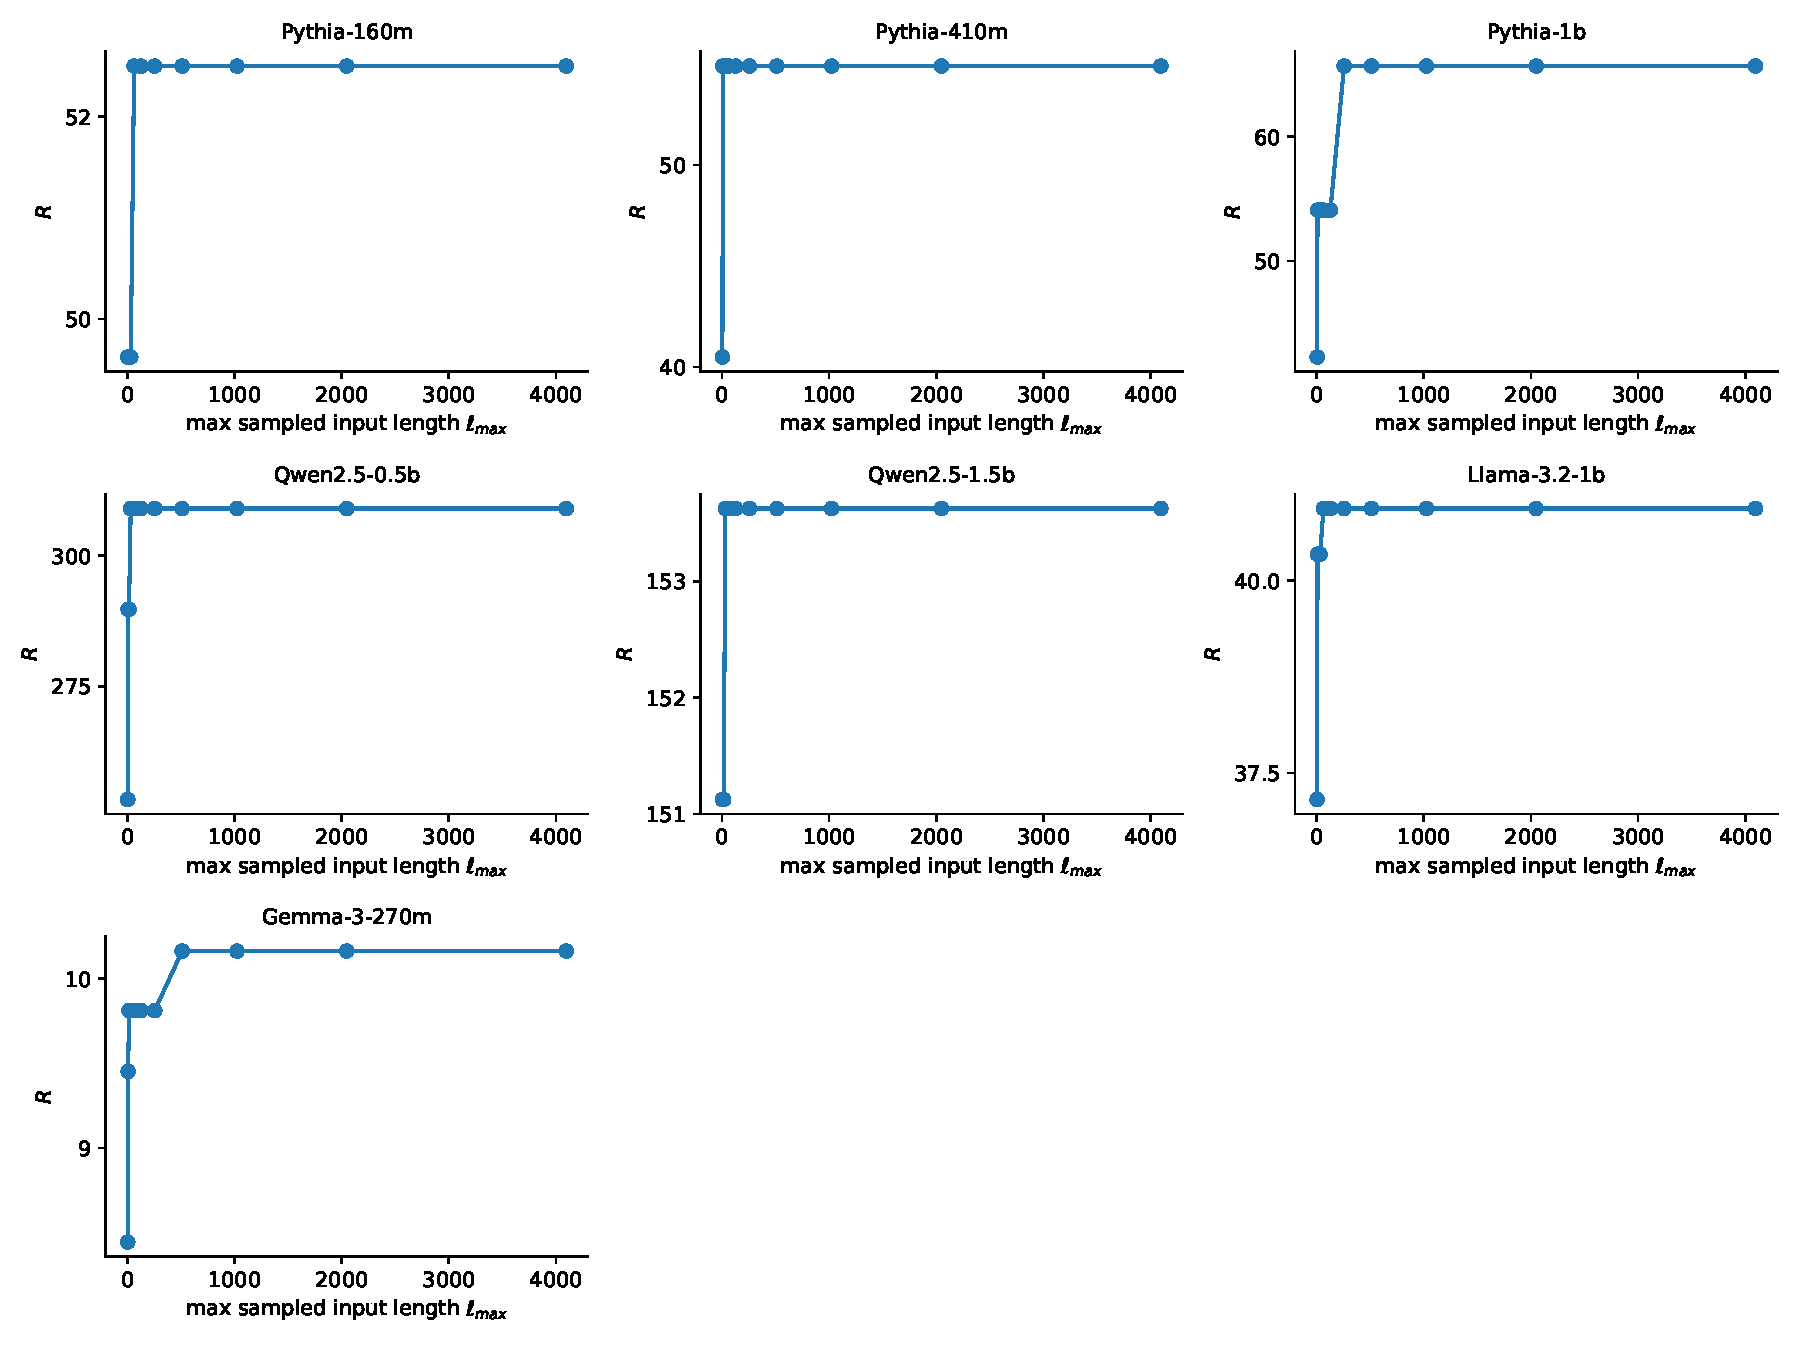
\includegraphics[width=0.7\linewidth]{Images/Rwrtell_max.pdf}
    \caption{Maximal radius $R$ of the internal representations of the transformer for various input lengths.}
    \label{fig:radius}
\end{figure}




\section{Mean-Field Transformers}\label{app:mean_field}

To extend the action of transformers beyond empirical measures to general probability distributions, we introduce the notion of pushforward. 
\begin{definition}[\citet{santambrogio2015optimal}]
    Given a probability measure $\mu$ on \(\mathbb{R}^d \) and a measurable map \( \varphi: \mathbb{R}^d \to \mathbb{R}^d \), the \emph{pushforward} of \( \mu \) by \( \varphi \), denoted by \( \varphi_{\sharp} \mu \), is the probability   measure defined on Borel sets \( B \subset \mathbb{R}^d \) by
\[
(\varphi_{\sharp} \mu)(B) := \mu(\varphi^{-1}(B)).
\]
\end{definition}

Intuitively, \( \varphi_{\sharp} \mu \) is obtained by transporting mass from each point \( x \) to its image \( \varphi(x) \), preserving total measure. We now define a mean-field transformer, denoting \( \mathcal{P}_{\mathrm c}(\mathbb{R}^d) \) the set of compactly supported probability measures on \( \mathbb{R}^d \).

\begin{definition}[Mean-Field Self-Attention~\citep{Castin_V_2024_p-icml_lipschitz}]
\label{def:meanfield_attention}
The mean-field generalization $F$ of any self-attention layer---parameterized by projection matrices $\mathbf{W}_{\mathrm q}$, $\mathbf{W}_{\mathrm k}$, $\mathbf{W}_{\mathrm v}$, and $\mathbf{W}_{\mathrm o}$ as defined in Definition~\ref{def:attention}---is defined by
\[
F: \mu \in \mathcal{P}_{\mathrm c}(\mathbb{R}^d) \mapsto (\Gamma_\mu)_{\sharp} \mu \in \mathcal{P}_{\mathrm c}(\mathbb{R}^d),\quad\mbox{where}
\]
\[
\Gamma_\mu(\mathbf x) := \sum_{i=1}^{h}\frac{\int  \mathbf{W}_{\mathrm o}^i \mathbf{W}_{\mathrm v}^i \mathbf y \cdot \exp\big((\mathbf{W}_{\mathrm k}^i \mathbf{y})^\top \mathbf{W}_{\mathrm q}^i \mathbf{x} \big) \, \mathrm{d} \mu(\mathbf y)}{\int \exp\big((\mathbf{W}_{\mathrm k}^i \mathbf{y})^\top \mathbf{W}_{\mathrm q}^i \mathbf{x} \big) \, \mathrm{d} \mu(\mathbf y)}.
\]

Mean-field self-attention $F$ generalizes discrete self-attention $\operatorname{Att}$ in the sense that for any input \(\mathbf X \in \mathbb{R}^{d\times m} \), we have \( F(\mathrm{M}(\mathbf X)) = \mathrm{M}(\operatorname{Att}(\mathbf X,\mathbf X)) \).
\end{definition}

\begin{definition}[Mean-Field Transformer Layer]

Similarly, any transformer layer $\tau$, with MLP layer $\operatorname{MLP}$ and mean-field self-attention layer defined by $\Gamma_\cdot$, has the following mean-field generalization $T$.
\[
T: \mu \in \mathcal{P}_{\mathrm c}(\mathbb{R}^d) \mapsto (\Delta_\mu)_{\sharp} \mu \in \mathcal{P}_{\mathrm c}(\mathbb{R}^d),\quad\mbox{where}
\]
\[
\Delta_\mu(\mathbf x) := \operatorname{MLP}(\Gamma_\mu(\mathbf x)+\mathbf x).
\]

Similarly to mean-field self-attention, a mean-field transformer layer $T$ generalizes a discrete transformer layer $\tau$ in the sense that for any input \(\mathbf X \in \mathbb{R}^{d\times m} \), we have \( T(\mathrm{M}(\mathbf X)) = \mathrm{M}(\tau(\mathbf X)) \)~\citep{meyer2025memorylimitationsprompttuning}. With a slight abuse of notation, we use the same symbol $\tau$ to denote a transformer and its mean-field counterpart.

\begin{remark}[Mean-Field Generalization of Masked Attention]
    We can easily generalize the mean-field framework to masked attention by augmenting the support of the probability measures to $[0,1]\times\mathbb R^d$, as adding $[0,1]$ allows to encode the position of every token~\citep{Castin_V_2024_p-icml_lipschitz}.
\end{remark}

    
\end{definition}



\section{Packing Number}\label{app:packing}

Recall the definition of packing number.

\defpacking*

In this section, we provide upper and lower bounds on the packing number of the sets we are studying.

\subsubsection*{The finite prompt length setting}

We use the following main result to analyze the setting of bounded length prompts.

\begin{restatable}{proposition}{prppackingfinite}\label{prp:packing_finite}
    Let $d\in\mathbb N$, $r>0$, and \( \varepsilon > 0 \). Then
    \[
        \Big(\frac{r}\varepsilon\Big)^d\leq\mathcal{P}(B^d(0,r), \|\cdot\|,\varepsilon)\leq\Big(1+\frac{2r}\varepsilon\Big)^d
    \]
\end{restatable}

\subsubsection*{The mean-field framework}

We obtain similar results for the study of prompts of arbitrary length in the mean-field framework. Let $\mathcal G:=\operatorname{Im}(\mathrm{M})=\{\mathrm M(\mathbf X),\mathbf X\in\mathbb R^{d\times m},m\in\mathbb N\}$ be the set of discrete probability measures on the token embeddings of dimension $d$ as defined in Section~\ref{sec:mean-field}.

\begin{proposition}\label{prp:packing_infinite}
    For any $q\ge1,\varepsilon>0$, there exists $C>0$ such that
    \[\operatorname{ln}\Big(\frac1C\Big)+\frac1{\varepsilon^d}\le\operatorname{ln} \mathcal P(\mathcal{G}, W_q,2\varepsilon) \leq \Big(1+\frac{4r}\varepsilon\Big)^d \operatorname{ln}\Big(e + \frac{e \, (2r)^q}{\varepsilon^q}\Big),\]
\end{proposition}

\subsection{Proofs}

A central result we need is the volume of the $d$-dimensional ball.

\begin{lemma}[\citet{vol_unit_ball,vol_ball}]\label{lem:Wang}
Assume $p_1, \ldots, p_d > 0$. 
The volume of the generalized unit ball in $\mathbb{R}^d$
\[
B_{p_1 p_2 \cdots p_d}^d
= \left\{ \mathbf{x} = (x_1, \ldots, x_d) \;:\;
|x_1|^{p_1} + \cdots + |x_d|^{p_d} \leq 1 \right\},
\]  is equal to
\[
\operatorname{Vol}\big(B_{p_1 p_2 \cdots p_d}^d\big)=2^d \, \frac{\Gamma\!\left(1+\tfrac{1}{p_1}\right)\cdots \Gamma\!\left(1+\tfrac{1}{p_d}\right)}
{\Gamma\!\left(\tfrac{1}{p_1} + \tfrac{1}{p_2} + \cdots + \tfrac{1}{p_d} + 1\right)} \, .
\]
Note that we can take some of the $p_i$'s to be $+\infty$ with the convention $\frac1{+\infty}=0$.

In particular, the volume of the $l_p$ ball of radius $r$ is
\[
\operatorname{Vol}\!\big(B_p^d(0,r)\big)
= (2r)^d\frac{ \, \Gamma\!\left(\tfrac{p+1}{p}\right)^d}{\Gamma\!\left(\tfrac{p+d}{p}\right)}.
\]
And the one corresponding to the $l_\infty$ norm is
\[
\operatorname{Vol}\!\big(B_\infty^d(0,r)\big)
= (2r)^d.
\]
\end{lemma}

Proposition~\ref{prp:packing_finite} can be proved using known bounds for the packing number of a general bounded set $K$, depending on the volume of $K$.

\begin{lemma}[{\citet[Proposition~4.2.10]{Vershynin_R_2018_b_covering-number}}]\label{lem:Vershynin}
Let $d\in\mathbb N$, \( K \subset \mathbb{R}^d \) and \( \varepsilon > 0 \). Then,
\begin{align*}
    \frac{|K|}{|\varepsilon B^d(0,1)|} 
\ \leq\ \mathcal{P}(K, \|\cdot\|, \varepsilon),\quad\mbox{and}\\ 
\ \ \mathcal{P}(K, \|\cdot\|, \varepsilon) 
\ \leq\ \frac{|K + (\varepsilon/2)B^d(0,1)|}{|(\varepsilon/2) B^d(0,1)|}.
\end{align*}
\end{lemma}

We can then deduce Proposition~\ref{prp:packing_infinite} from the following two lemmas.

\begin{lemma}[{\citet[Lemma~4.b]{Nguyen}}]
    For any $q\ge1,\varepsilon>0$,
    \[\operatorname{ln} \mathcal P(\mathcal{G}, W_q,4\varepsilon) \leq \mathcal P(\Theta, \|\cdot\|_q, \varepsilon) \operatorname{ln}\Big(e + \frac{e \, \mathrm{Diam}(\Theta)^q}{\varepsilon^q}\Big),\]
    with $\Theta=B^d(0,r)$ and $e=\exp(1)$.
\end{lemma}


\begin{lemma}[{\citet[Proposition~3.6]{meyer2025memorylimitationsprompttuning}}]\label{prp:klo}
   For any $q\ge1,\varepsilon>0$, there exists $C>0$ such that
    \[
    \mathcal{P}(\mathcal G, W_q,\varepsilon)\ge\frac1C\exp(\frac1{\varepsilon^d}).
    \]
\end{lemma}

\section{Permutation-Invariant Norms and Wasserstein Distances}\label{app:wasserstein}

In this section, we discuss the Wasserstein distance, and specifically how the Wasserstein distance between two empirical measures $\mathrm M(\mathbf X)$ and $\mathrm M(\mathbf Y)$ relates to the classical distance $\|\mathbf X-\mathbf Y\|$. This allows us to study the validity of Assumption~\ref{ass:wasserstein}.

\begin{definition}[Wasserstein Distance~\citep{santambrogio2015optimal}]\label{def:wasserstein}
    For $q\geq1$, the $\ell_q$ Wasserstein distance on $\mathcal{P}_{\mathrm c}(\mathbb{R}^d)$ is given by
    \[
    W_q(\mu, \nu) = \left( \inf_{\pi \in \Pi(\mu, \nu)} \int \|x - y\|^q \, \mathrm{d}\pi(x, y) \right)^{1/q},
    \]
    for \( \mu, \nu \in \mathcal{P}_{\mathrm c}(\mathbb{R}^d) \), where \( \Pi(\mu, \nu) \) is the set of couplings between \( \mu \) and \( \nu \), {\it i.e.} of probability measures \( \pi \in \mathcal{P}(\mathbb{R}^d \times \mathbb{R}^d) \) such that \( \int \pi(\cdot, y)\, \mathrm{d}y = \mu \) and \( \int \pi(x, \cdot)\, \mathrm{d}x = \nu \).

    The $\ell_\infty$ Wasserstein distance is defined as the limit of the $W_q$ distance as $q$ goes to infinity.
    \[
    W_\infty(\mu, \nu) = \lim_{q\rightarrow\infty}W_q(\mu,\nu)
    \]

    In particular, two sequences $\mathbf{X},\mathbf{Y}\in \mathbb{R}^{d\times n}$ of equal length $n$ are of Wasserstein distance

    \begin{align*}
    &W_q(\mathrm{M}(\mathbf X), \mathrm{M}(\mathbf Y))
    = \left( \min_{\pi \in S_n} \frac{1}{n} \sum_{i=1}^n \| X_{:,i} - Y_{:,\pi(i)} \|^q \right)^{1/q},\\
    &W_\infty(\mathrm{M}(\mathbf X), \mathrm{M}(\mathbf Y))
    = \min_{\pi \in S_n} \, \max_{i=1,\dots,n} \| X_{:,i} - Y_{:,\pi(i)} \|.
    \end{align*}


\end{definition}


The permutation invariance of the mean-field transformer architecture prompts us to consider permutation invariant versions of the $\ell_p$ and $\ell_\infty$ distances.

\begin{definition}
    Consider two sequences $\mathbf{X},\mathbf{Y}\in \mathbb{R}^{d\times n}$ of equal length $n$.
    For $\pi\in S_n$, let $\mathbf{Y}_\pi = (\mathbf Y_{:,\pi(1)},\dots,\mathbf Y_{:,\pi(n)})$. Then
    \begin{align}
    d_q(\mathbf{X},\mathbf{Y})
    &= \min_{\pi\in S_n} \,\big\|\, \mathbf{X} - \mathbf{Y}_\pi \,\big\|_{q}, \nonumber
    \quad 1\le q<\infty, \\
    d_\infty(\mathbf{X},\mathbf{Y})\nonumber
    &= \min_{\pi\in S_n} \,\big\|\, \mathbf{X} - \mathbf{Y}_\pi \,\big\|_{\infty},
    \end{align}
    where $S_n$ denotes the set of permutations of $[n]$.
\end{definition}

We can now relate Wasserstein distance between empirical measures and classical distance.

\begin{proposition}\label{prp:relation_wass-classical}
     Consider two sequences $\mathbf{X},\mathbf{Y}\in \mathbb{R}^{d\times n}$ of equal length $n$. Then,
    \begin{align}
    W_q(\mathrm{M}(\mathbf{X}),\mathrm{M}(\mathbf{Y}))
    &= n^{-1/q}\, d_q(\mathbf{X},\mathbf{Y}), \quad 1\le q<\infty, \nonumber\\
    W_\infty(\mathrm{M}(\mathbf{X}),\mathrm{M}(\mathbf{Y}))
    &= d_\infty(\mathbf{X},\mathbf{Y}).\nonumber
    \end{align}
\end{proposition}

Notice that bounding the Wasserstein distance between two empirical measures $\mathrm M(\mathbf X)$ and $\mathrm M(\mathbf Y)$ does not directly bound the distance between $\mathbf X$ and $\mathbf Y$. The latter bound depends on the lengths of both vectors. Therefore, a finite precision on vectors does not directly imply a finite Wasserstein precision (that is Assumption~\ref{ass:finite} does not directly imply Assumption~\ref{ass:wasserstein}).

However, one can clearly see that Assumption~\ref{ass:finite} is very weak for large vectors. Indeed, if a transformer cannot distinguish two vectors whose $\ell_1$-distance is at most $\varepsilon$ when their length is $1$, then for vectors of length $n$, this tolerance scales roughly as $n\varepsilon$. In other words, the same absolute $\ell_1$-precision becomes increasingly coarse as the vector length grows: small perturbations distributed across many coordinates can yield an $\ell_1$ deviation of order $n\varepsilon$ while remaining imperceptible to the model.

Of course, assuming a uniform $\varepsilon$-precision in the $\ell_1$ norm is overly restrictive. Yet, the argument above suggests that for some $q\ge1$, the effective distinguishability of the model may scale as $n^{-1/q}\varepsilon$. Therefore, Proposition~\ref{prp:relation_wass-classical} provides theoretical support for Assumption~\ref{ass:wasserstein}: a finite vector precision naturally induces a finite Wasserstein precision when the appropriate scaling with $n$ and $q$ is taken into account.

\section{Arbitrary Prompt Length via Elementary Operations}\label{app:eo}

Contrary to Assumption~\ref{ass:finite}, Assumption~\ref{ass:wasserstein} is non-trivial. We show in this section that it can be replaced by a much weaker assumption, pertaining to what we call elementary operations.

\begin{definition}[Elementary Operations on a Sequence of Vectors]
    Let $\mathbf X=[\mathbf x_1,\ldots,\mathbf x_n]$ be a sequence of $n$ vectors. An elementary operation on $\mathbf X$ consists in duplicating or removing one of its tokens. 
\end{definition}

\begin{assumption}[Elementary Operation Precision of a Transformer]\label{ass:eo}
    Let $\tau$ be a transformer. There exists a constant $p\in\mathbb N$ such that, if a sequence of tokens $\mathbf Y$ can be recovered from another sequence $\mathbf X\in\mathbb R^{d\times n}$ of length $n$ through at most $\frac n p$ elementary operations, then $\tau$ cannot distinguish between $\mathbf Y$ and $\mathbf X$. We say that $\frac1p$ is the elementary operation precision (e.o. precision) of $\tau$.
\end{assumption}

This assumption states that a transformer $\tau$ is insensitive to small structural edits of its input sequence. The only allowed operations are token deletions and duplications---no arbitrary modifications of token content. It is therefore reasonable to expect that if $\mathbf{Y}$ differs from $\mathbf{X}$ by only a small fraction of such operations, then $\tau$ produces nearly identical representations. Although we do not specify the exact constant $p$, the claim clearly fails for large perturbations (e.g., modifying half the tokens) and is trivially true for extremely small ones (e.g., $0.001\%$ of the tokens). Hence, it is highly plausible that there exists a non-trivial fraction $1/p$ for which Assumption~\ref{ass:eo} holds.

Under Assumption~\ref{ass:eo}, we can obtain an upper bound on the number of different inputs a given transformer $\tau$ can distinguish between, and hence on the amount of distinct output sequences it can access. This upper bound is a function of both the e.o. precision $p$ of the transformer, and the number of distinct input values $D$ it can distinguish between. If we consider a hard prompt transformer [Definition~\ref{def:hard_prompt}] without positional embedding, then $D=|\mathcal V|$. In general, we can take $D=(\frac r \varepsilon)^d$, where $\varepsilon$ is the standard precision of $\tau$ and $r$ is its embedding radius.

\begin{restatable}{theorem}{thmeo}\label{thm:eo}
    There exists an upper bound $f(p,D)$ on the number of sequences of tokens that are accessible by a transformer $\tau$ with elementary operation precision $\frac1p$.
\end{restatable}


\begin{proof}
    We showed that the input space of $\tau$ is exactly the set of empirical distributions over $[D]$, which is a subset of $\mathbb N^D$. That is the transformer maps to the same image two inputs $\mathbf x$ and $\mathbf y$ satisfying $\exists q\in\mathbb Q,\mathbf x=q\mathbf y$. We denote by $\mathcal R$ and $\bar{\mathbf x}$ the associated equivalence relation and equivalence classes:
    \begin{itemize}
        \item $\forall \mathbf x,\mathbf y\in\mathbb N^D,\mathbf x\mathcal R \mathbf y\iff\exists q\in\mathbb Q,\mathbf x=q\mathbf y$.
        \item $\forall\mathbf x\in\mathbb N^D,\bar{\mathbf x}=\{\mathbf y\in\mathbb N^D\colon \mathbf x\mathcal R\mathbf y\}$.
    \end{itemize}
    Then the input space of $\tau$ is exactly $\mathbb N^D/\mathcal R=\{\bar{\mathbf x}\colon\mathbf x\in\mathbb N^D\}$. An important thing to note is that in $\mathbb N^D/\mathcal R$, the length of an empirical distribution $\mathbf x$ is simply $\|\mathbf x\|_1$, and an elementary operation on $\mathbf x$ amounts to adding or subtracting $1$ to a non-zero coefficient of $\mathbf x$.
    
    Take the basis $\mathcal B=\{\mathbf x\in\mathbb N^D\colon\|\mathbf x\|_\infty<b\}$. Theorem~\ref{thm:eo} is a direct consequence of the fact that every vector $\bar{\mathbf x}\in\mathbb N^D/\mathcal R$ is at most $g(b,D)\|\mathbf x\|_1$ elementary operations away from a basis vector for some function $g$. Then, we conclude the proof by choosing $b$ such that $g(b,D)\le\frac1p$, and obtain $f(p,D)=|\mathcal B|=b^D$.
    
    A very straightforward way of proving this result is presented in this section. We obtain $g(b,D)=\frac{D}{2(b-2)}$ and $b=\big\lceil\frac {pD}2\big\rceil$ in Lemma~\ref{lem:eo}. We provide in Appendix~\ref{app:eo} more complicated proofs leading to tighter bounds.
\end{proof}

\begin{lemma}\label{lem:eo}
    Let $\mathbf x\in\mathbb N^D$. There exists $\bar{\mathbf y}\in\bar{\mathcal B}\coloneqq\{\bar{\mathbf y}\colon\mathbf y\in\mathcal B\}$ such that $\|\mathbf x-\mathbf y\|_1\leq \frac{D\|\mathbf x\|_1}{2(b-2)}$.
\end{lemma}

\begin{proof}
     Let $\mathbf x=(x_1,\ldots,x_D)\in\mathbb N^D$. Without loss of generality, assume that $x_1\le\ldots\le x_D$. Let $l\in\mathbb N$ be the quotient of the euclidean division of $x_D$ by $b-2$: $l(b-2)\le x_D<l(b-1)$. Then there exists $\mathbf y=(y_1,\ldots,y_D)\in\mathbb N^D$ such that $\|\mathbf x-\mathbf y\|_1\le D\big\lfloor\frac l2\big\rfloor$ and $\forall i\in[D],l|y_i$ (every $y_i$ is the closest multiple of $l$ to $x_i$). 

     Clearly, $\frac1l\mathbf y\in\mathcal B$ and ${\mathbf y}\mathcal R(\frac1l{\mathbf y})$. Hence $\bar{\mathbf y}=\frac1l\bar{\mathbf y}\in\bar{\mathcal B}$.

     Finally, $l\le\frac{x_D}{b-2}\le\frac{\|\mathbf x\|_1}{b-2}$ so $\|\mathbf x-\mathbf y\|_1\le\frac{D\|\mathbf x\|_1}{2(b-2)}$.
\end{proof}

\subsection{Tighter Bounds for Theorem~\ref{thm:eo}}

\thmeo*

Recall that to prove Theorem~\ref{thm:eo}, for every $p\in\mathbb N$ we obtain a basis $\mathcal B=\{\mathbf x\in\mathbb N^D\colon\|\mathbf x\|_\infty<b\}$ for some $b\in\mathbb N$ that is $\frac1p$-dense in $\mathbb N^D$ in the sense that
\[\forall\mathbf x\in\mathbb N^D,\exists\mathbf y\in\mathbb N^D,\begin{cases}
\bar{\mathbf y}\in\bar{\mathcal B},\\
\|\mathbf x-\mathbf y\|_1\leq\frac{\|\mathbf x\|_1}p.
\end{cases}\]
Then, clearly $f(p,D)\leq|\mathcal B|=b^D$.

\begin{remark}
    Note that the last equality $f(p,D)\leq|\mathcal B|=b^D$ leaves room for improvement as $f(p,D)\leq|\bar{\mathcal B}|<|\mathcal B|=b^D$.
\end{remark}

In Lemma~\ref{lem:eo}, we propose $b=\big\lceil\frac {pD}2\big\rceil$ for the basis radius. Let us show that $b=2p$ suffices.

\begin{lemma}
    Let $\mathbf x\in\mathbb N^D$. There exists $\bar{\mathbf y}\in\bar{\mathcal B}\coloneqq\{\bar{\mathbf y}\colon\mathbf y\in\mathcal B\}$ such that $\|\mathbf x-\mathbf y\|_1\leq \frac{2\|\mathbf x\|_1}{b}$.
\end{lemma}

\begin{proof}
    For the purpose of this proof, we introduce the distance $\mathrm d$ on $\mathbb N^D/\mathcal R$ defined as $\mathrm d(\bar{\mathbf x},\bar{\mathbf y})=\min_{\mathbf x\in\bar{\mathbf x},\mathbf y\in\bar{\mathbf y}}\|\mathbf x-\mathbf y\|_1$.

    Let $\mathbf x=(x_1,...,x_{D})\in\mathbb N^D$. By considering separately the cases where $\min_{i\in[D]}x_i\leq\frac{\|\mathbf x\|_1}{b^2}$ and $\min_{i\in[D]}x_i>\frac{\|\mathbf x\|_1}{b^2}$, we can show that there exists $\mathbf y^1=(0,\ldots,0,y,n_1y,\ldots,n_ky)\in\mathbb N^D$ such that $\mathrm d(\bar{\mathbf x},\overline{\mathbf y^1})\leq \frac{\|\mathbf x\|_1}{b}$.
    
    Without loss of generality, assume that $n_1\leq\ldots\leq n_{k}$. If $n_k\leq b$, then $\overline{\mathbf y^1}=\overline{(0,\ldots,0,1,n_1,\ldots,n_k)}\in\bar{\mathcal B}$. Else, consider $\mathbf y^2=(0,\ldots,0,0,n_1y,\ldots,n_ky)\in\mathbb N^D$ which satisfies $\|\mathbf y^1-\mathbf y^2\|_1=y= \frac{\|\mathbf y^1\|_1}{1+n_1+\cdots+n_k}<\frac{\|\mathbf y^1\|_1}{1+kb}$.

    We can conclude by induction.
\end{proof}

\section{Theoretical Slope of the Cramming Task for Various Supports}
\label{app:shapes}

We describe how we obtain the formulas for the various slopes in the following subsections. First, let us introduce a few useful notations and equations.

Let $\mathcal D$ be the distribution over the volume proportion $\frac{|\mathcal{E}_t|}{|\mathcal E|}$ of the next-token cells. That is $\mathcal D(I)=\frac1{|\mathcal V|}\sum_{t\in\mathcal V}\mathbf 1_{\frac{|\mathcal{E}_t|}{|\mathcal E|}\in I}$ for all $I\subset\mathbb R^+$. We can approximate the distribution over the volume fractions $\frac{|\mathcal{E}_{\mathbf t}|}{|\mathcal E|}$ of the sequences of length $n$, $\mathbf t\in\mathcal V^n$ by 
\begin{align}\label{eq:assumption}
    \mathcal D_n(I)&=\frac1{|\mathcal V|^n}\sum_{\mathbf t\in\mathcal V^n}\mathbf 1_{\frac{|\mathcal{E}_{\mathbf t}|}{|\mathcal E|}\in I}\nonumber\\
    &\simeq\frac1{|\mathcal V|^n}\sum_{\mathbf t\in\mathcal V^n}\mathbf 1_{(\prod_{i=1}^n\frac{|\mathcal{E}_{\mathbf t_i}|}{|\mathcal E|})\in I}\nonumber\\
&= \mathcal D^n(I),
\end{align}

where $\mathcal D^n$ denotes the distribution of the product of $n$ variables $X_1,...,X_n\overset{\text{iid}}{\sim}\mathcal D$. Then, at least half of the token sequences of length $n$ are inaccessible if $\mathrm{Med}(\mathcal D^n)\leq\frac{1}{\mathcal{P}(\mathcal E,\|\cdot\|,\varepsilon)}$, where $\mathrm{Med}(\mathcal D^n)$ denotes the median of $\mathcal D^n$. Note that in the setting of Corollary~\ref{thm:finite}, $\mathcal D$ is equal to the Dirac distribution $\delta_{\frac{1}{|\mathcal V|}}$, and we recover the slope $\frac{\ln(\mathcal{P}(\mathcal E,\|\cdot\|,\varepsilon))}{\ln(|\mathcal V|)}$ from 

\begin{align}\label{eq:slope}
    \mathrm{Med}(\mathcal D^n)\leq\frac{1}{\mathcal{P}(\mathcal E,\|\cdot\|,\varepsilon)}\quad&\iff\quad\frac1{|\mathcal V|^n}\leq\frac{1}{\mathcal{P}(\mathcal E,\|\cdot\|,\varepsilon)}\nonumber\\
    &\iff\quad n\geq\frac{\ln(\mathcal{P}(\mathcal E,\|\cdot\|,\varepsilon))}{\ln(|\mathcal V|)}.
\end{align}

\begin{remark}
    In Eq.~\ref{eq:assumption}, we assume conditional independence of next-token cells: for any realized prefix, the distribution of subsequent cell volumes within the selected cell is again $\mathcal{D}$. 
    Although strong, this assumption is conservative: we hypothesize that adding context reduces the number of plausible next tokens, making the next-token distribution sharper than the marginal and thus yielding more variance in the volume cells than $\mathcal{D}$.
    Under this view, the i.i.d.\ model $\mathcal{D}^n$ is expected to overestimate typical continuation volumes and can be interpreted as an upper bound.
\end{remark}

\subsection{When the Support Is a Ball}

\begin{proposition}
    Let $B^{d\times m}(0,r)\supset\mathcal E$ be an enclosure of the embedding support. Then the slope of the Cramming Task satisfies $C\leq d\frac{\operatorname{ln}(1+\frac {2r}{\varepsilon})}{\operatorname{ln}(|\mathcal V|)}$.
\end{proposition}

\begin{proof}
    This is a simple corollary of Equation~\ref{eq:slope} and Proposition~\ref{prp:packing_finite}.
\end{proof}

\subsection{When the Support Is a Cone}

Let $n\ge 2$, $r>0$, and $\delta\in(0,\pi)$. Define the (infinite) cone of angle $\delta$
\[
C_\delta:=\Bigl\{\mathbf x\in\mathbb R^{n}:\ \mathbf x_1\tan(\delta/2)>\sqrt{\sum_{i=2}^n\mathbf x_i^2}\Bigr\},
\]
and its truncation by the Euclidean ball $B^d(0,r):=\{\mathbf x\in\mathbb R^d:\ \sqrt{\sum_{i=1}^d\mathbf x_i^2}<r\}$:
\[
C_{\delta,r}:=C_\delta\cap B^d(0,r).
\]

\begin{proposition}
    Let $C_{\delta,r}^m\supset\mathcal E$ be an enclosure of the embedding support. Then the slope of the Cramming Task satisfies \[C\leq \frac 1{\operatorname{ln}(|\mathcal V|)}\operatorname{ln}\Bigg(\big(1+\frac{2r}\varepsilon\big)^d\frac{\Gamma(\frac{d+2}2)} {2r\Gamma(\frac{3}2)\Gamma(\frac{d+1}2)}
    \Bigg[\frac{1}{d}\,\sin^{\,d-1}\!\Bigl(\frac{\delta}{2}\Bigr)\cos\!\Bigl(\frac{\delta}{2}\Bigr)
+\frac{1}{2}\Bigl(B\!\Bigl(\tfrac12,\tfrac{d+1}{2}\Bigr)-B\!\Bigl(\cos^2(\tfrac{\delta}{2});\tfrac12,\tfrac{d+1}{2}\Bigr)\Bigr)\Bigg]\Bigg),\] where $B(a,b)=\int_0^1 t^{a-1}(1-t)^{b-1}\,dt$ is the Beta function, and
$B(x;a,b)=\int_0^x t^{a-1}(1-t)^{b-1}\,dt$ is the incomplete Beta function.
\end{proposition}

\begin{proof}

\begin{lemma}\label{lem:cone_vol}
The volume of the $d$-dimensional cone of angle $\delta$ and radius $r$ satisfies
\[
|C_{\delta,r}|
=\omega_{d-1}\,r^d\left[
\frac{1}{d}\,\sin^{\,d-1}\!\Bigl(\frac{\delta}{2}\Bigr)\cos\!\Bigl(\frac{\delta}{2}\Bigr)
+\frac{1}{2}\Bigl(B\!\Bigl(\tfrac12,\tfrac{d+1}{2}\Bigr)-B\!\Bigl(\cos^2(\tfrac{\delta}{2});\tfrac12,\tfrac{d+1}{2}\Bigr)\Bigr)
\right],
\]
where $\omega_{d-1}:=|B^{d-1}(0,1)|$ is the volume of the unit ball in $\mathbb R^{d-1}$.
\end{lemma}

\begin{proof}[Proof of Lemma~\ref{lem:cone_vol}]
    \textbf{Step 1: Scaling Reduction.}
For any $r>0$, the change of variables $\mathbf x=r\mathbf y$ gives
\[
|C_\delta\cap B^d(0,r)|
=\int_{\mathbb R^d}\mathbf{1}_{C_\delta}(\mathbf x)\mathbf{1}_{B^d(0,r)}(\mathbf x)\,d\mathbf x
=\int_{\mathbb R^d}\mathbf{1}_{C_\delta}(r\mathbf y)\mathbf{1}_{B^d(0,1)}(\mathbf y)\,r^d\,d\mathbf y
=r^d|C_\delta\cap B^d(0,1)|,
\]
since $C_\delta$ is a cone (i.e.\ $\mathbf y\in C_\delta\iff r\mathbf y\in C_\delta$ for $r>0$).
Thus it suffices to compute $|C_\delta\cap B^d(0,1)|$.

\textbf{Step 2: Disjoint Decomposition.}
Write, as shown in Figure~\ref{fig:cone},
\[
E_\delta:=(C_\delta\cap B^d(0,1))\cap\{0<\mathbf x_1<\cos(\delta/2)\},\qquad
F_\delta:=(C_\delta\cap B^d(0,1))\cap\{\cos(\delta/2)<\mathbf x_1<1\}.
\]

\begin{figure}
    \centering
    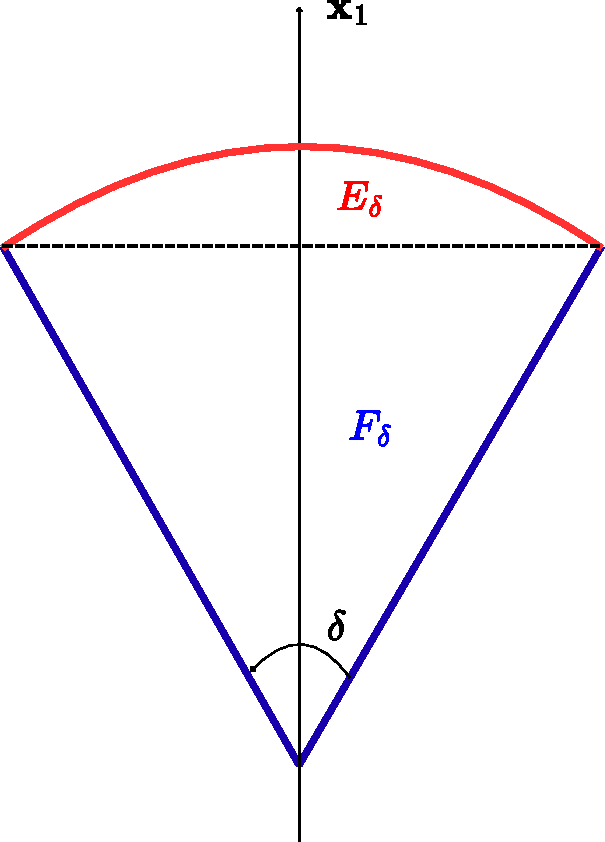
\includegraphics[width=0.2\linewidth]{Images/Cone.pdf}
    \caption{Decomposition of the cone in $E_\delta$ and $F_\delta$.}
    \label{fig:cone}
\end{figure}

Then $C_\delta\cap B^d(0,1)=E_\delta\;\dot\cup\;F_\delta$ up to a null set (the slice $\mathbf x_1=\cos(\delta/2)$),
so
\[
|C_\delta\cap B^d(0,1)|=|E_\delta|+|F_\delta|.
\]

\textbf{Step 3: Volume of the Conical Part $E_\delta$.}
Fix $\rho\in(0,\cos(\delta/2))$. On the hyperplane $\{\mathbf x_1=\rho\}$, we have
\[
\sqrt{\sum_{i=2}^d\mathbf x_i^2}<\mathbf x_1\tan(\delta/2)=\mathbf \rho\tan(\delta/2).
\]
Since $\rho<\cos(\delta/2)$, we obtain
\[
\rho\tan(\delta/2)\le \cos(\delta/2)\tan(\delta/2)=\sin(\delta/2).
\]
Hence $\sum_{i=1}^d\mathbf x_i^2=\rho^2+\sum_{i=2}^d\mathbf x_i^2<\rho^2+\sin^2(\delta/2)\le 1$.

So the ball constraint $\sqrt{\sum_{i=1}^d\mathbf x_i^2}<1$ is inactive on these slices and
\[
\{\mathbf x_1=\rho\}\cap E_\delta=\{\rho\}\times B^{d-1}(0,\rho\tan(\delta/2)).
\]
Thus,
\[
|E_\delta|
=\int_{0}^{\cos(\delta/2)} |B^{d-1}(0,\rho\tan(\delta/2))|\,d\rho
=\int_{0}^{\cos(\delta/2)} \omega_{d-1}\bigl(\rho\tan(\delta/2)\bigr)^{d-1}\,d\rho.
\]
Evaluating the integral yields
\[
|E_\delta|
=\omega_{d-1}\tan^{d-1}(\delta/2)\int_{0}^{\cos(\delta/2)}\rho^{d-1}\,d\rho
=\frac{\omega_{d-1}}{d}\tan^{d-1}(\delta/2)\cos^d(\delta/2)
=\frac{\omega_{d-1}}{d}\sin^{d-1}(\delta/2)\cos(\delta/2).
\]

\textbf{Step 4: Volume of the Spherical-Cap Part $F_\delta$.}
Fix $\rho\in(\cos(\delta/2),1)$. On the hyperplane $\{\mathbf x_1=\rho\}$, the ball constraint $\sqrt{\sum_{i=1}^d\mathbf x_i^2}<1$
is equivalent to $\sqrt{\sum_{i=2}^d\mathbf x_i^2}<\sqrt{1-\rho^2}$. For $\rho>\cos(\delta/2)$,
\[
\sqrt{1-\rho^2}<\sqrt{1-\cos^2(\delta/2)}=\sin(\delta/2)=\cos(\delta/2)\tan(\delta/2)
<\rho\tan(\delta/2),
\]
so the cone constraint is inactive on these slices: the ball provides the tighter bound.
Thus
\[
\{\mathbf x_1=\rho\}\cap F_\delta=\{\rho\}\times B^{d-1}(0,\sqrt{1-\rho^2}).
\]
Hence,
\[
|F_\delta|
=\int_{\cos(\delta/2)}^{1}|B^{d-1}(0,\sqrt{1-\rho^2})|\,d\rho
=\omega_{d-1}\int_{\cos(\delta/2)}^{1}\bigl(1-\rho^2\bigr)^{\frac{d-1}{2}}\,d\rho.
\]
Let $\tau=\rho^2$, so $d\rho=\frac{1}{2}\tau^{-1/2}\,d\tau$. Then
\[
|F_\delta|
=\frac{\omega_{d-1}}{2}\int_{\cos^2(\delta/2)}^{1}\tau^{-1/2}(1-\tau)^{\frac{d-1}{2}}\,d\tau
=\frac{\omega_{d-1}}{2}\left[
B\!\Bigl(\tfrac12,\tfrac{d+1}{2}\Bigr)
- B\!\Bigl(\cos^2(\tfrac{\delta}{2});\tfrac12,\tfrac{d+1}{2}\Bigr)
\right].
\]

\textbf{Step 5: Conclusion.}
Summing the two contributions,
\[
|C_\delta\cap B^d(0,1)|
=\omega_{d-1}\left[
\frac{1}{d}\sin^{d-1}\!\Bigl(\frac{\delta}{2}\Bigr)\cos\!\Bigl(\frac{\delta}{2}\Bigr)
+\frac{1}{2}\Bigl(B\!\Bigl(\tfrac12,\tfrac{d+1}{2}\Bigr)-B\!\Bigl(\cos^2(\tfrac{\delta}{2});\tfrac12,\tfrac{d+1}{2}\Bigr)\Bigr)
\right],
\]
and scaling gives the claimed formula for $|C_\delta\cap B^d(0,r)|=r^d|C_\delta\cap B^d(0,1)|$.
\end{proof}

The packing number of $C_{\delta,r}$ follows by symmetry (or using Lemma~\ref{lem:Vershynin}).

\begin{corollary}\label{cor:cone_pak}
    The packing number of the $d$-dimensional cone of angle $\delta$ and radius $r$ satisfies
    \[
    \mathcal{P}(C_{\delta,r}, \|\cdot\|_2,\varepsilon)\lesssim\frac{\Gamma(\frac{d+2}2)} {2r\Gamma(\frac{3}2)\Gamma(\frac{d+1}2)}
    \Bigg[\frac{1}{d}\,\sin^{\,d-1}\!\Bigl(\frac{\delta}{2}\Bigr)\cos\!\Bigl(\frac{\delta}{2}\Bigr)
+\frac{1}{2}\Bigl(B\!\Bigl(\tfrac12,\tfrac{d+1}{2}\Bigr)-B\!\Bigl(\cos^2(\tfrac{\delta}{2});\tfrac12,\tfrac{d+1}{2}\Bigr)\Bigr)\Bigg]\mathcal{P}(B^d(0,r), \|\cdot\|_2,\varepsilon)
    \]
\end{corollary}

Finally, we can conclude using Equation~\ref{eq:slope} and Proposition~\ref{prp:packing_finite}.

\end{proof}

\subsection{When the Support Is an Ellipsoid}

We use here the $l_\infty$ norm.

\begin{proposition}
    Let $\Big([x^{\mathrm{min}}_1,x^{\mathrm{max}}_1]\times\cdots\times [x^{\mathrm{min}}_d,x^{\mathrm{max}}_d]\Big)^m\supset\mathcal E$ be an enclosure of the embedding support. Then the slope of the Cramming Task satisfies $C\leq \frac{\sum_{i=1}^d\operatorname{ln}(1+\frac {x^{\mathrm{max}}_i-x^{\mathrm{min}}_i}{\varepsilon})}{\operatorname{ln}(|\mathcal V|)}$.
\end{proposition}

\begin{proof}
    This is a simple corollary of Equation~\ref{eq:slope} and Proposition~\ref{prp:packing_finite}.
\end{proof}

\section{Supplementary Experimental Results}

\subsection{Latent space constants for each model}


\begin{table*}[ht]
\centering
\begin{tabular}{lccccccc}
\toprule
 & \multicolumn{3}{c}{Pythia} & \multicolumn{2}{c}{Qwen-2.5} & Llama-3.2 & Gemma-3 \\[-0.5ex]
\cmidrule(r{2pt}l{2pt}){2-4}\cmidrule(r{2pt}l{2pt}){5-6}\cmidrule(r{2pt}l{2pt}){7-7}\cmidrule(r{2pt}l{2pt}){8-8}
 & 160M & 410M & 1B & 0.5B & 1.5B & 1B & 270M \\[-0.5ex]
\midrule
Hidden dimension $d$ & 768 & 1024 & 2048 & 896 & 1536 & 2048 & 640   \\
Vocabulary Size $|\mathcal{V}|$& 50304 & 50304 & 50304 & 151936 & 151936 & 128256 & 262144 \\
Radius $r$ &  63.62 &  54.90 &  65.68 &  309.00 & 153.62 & 41.06 &  10.74   \\
% Precision $\varepsilon$ &  3.10e-2 & 2.68e-2 & 3.21e-2 & 1.51e-1 & 7.50e-2 & 2.01e-2 & 5.24e-3 \\
Cone angle $\theta$ & 1.96 & 1.87 & 2.22 & 2.23 & 2.34 & 1.73 & 1.82  \\
\bottomrule
\end{tabular}
\vspace{1.0em}
\caption{Model constants used to estimate slope upper-bound ratios in Table~\ref{tbl:slope}. The dimensionality $d$ and vocabulary size $|\mathcal{V}|$ are determined by the model architecture, while $r$ and $\theta$ are estimated in Section~\ref{sec:support}. }
\label{tbl:constants}
\vspace{-1.5em}
\end{table*}

\subsection{Estimation of precision $\varepsilon$}
\label{app:epsilon}

\subsubsection{Fixed Precision}
We assume a finite numerical precision in transformer computations: inputs closer than a threshold $\varepsilon$ are effectively indiscernible. In practice, transformers are typically evaluated using half-precision floating-point arithmetic (fp16), which uses $k_{\max}=5$ exponent bits and $p=11$ bits of significand precision.\footnote{Transformers are often trained using Brain Floating Point (bf16), but since it has fewer precision bits ($p=8$), it implies a larger $\varepsilon$. We therefore use fp16 as a conservative choice.}
For numbers with exponent $k$, the spacing between representable values is $2^{k-p}$. Thus, two values at exponent $k$ become indistinguishable after rounding if their difference is below this spacing.

We use the standard interval definition of machine epsilon: the gap between $1$ and the next representable floating-point value, i.e. $\varepsilon = 2^{-10}$, as used by Pytorch~\citep{pytorchTypeInfo}. 
This definition lets us instantiate precision-dependent constants for fp16 and derive upper bounds on model slopes. 

\subsubsection{Variable Precision}

One could however argue that this definition is not precise: the precision should vary depending on the order of magnitude of the number being represented. To that end, we revise the upper bound of the packing number as follows.

Let $\mathcal E = [r_{\min}, r_{\max}]$ be the embedding space, where $0 < r_{\min} \le r_{\max}$ (by symmetry, we can easily extend to the setting where $\mathcal E=[-r_{\mathrm{max}}^{-},-r_{\mathrm{min}}^{-}]\cup[r_{\mathrm{min}}^{+},r_{\mathrm{max}}^{+}]$).

Define
$$
a = \lceil \log_2 r_{\min} \rceil,
\qquad
b = \lceil \log_2 r_{\max} \rceil.
$$
Then
$$
2^{a-1} < r_{\min} \le 2^a,
\qquad
2^{b-1} < r_{\max} \le 2^b.
$$

And
$$
[r_{\min}, r_{\max}]=
[r_{\min},2^a]
\cup
[2^a,2^{a+1}]
\cup \cdots \cup
[2^{b-1},r_{\max}].
$$
Hence, by subadditivity of the packing number,
$$
\mathcal P(\mathcal E)
\le
\mathcal P([r_{\min},2^a])
+\sum_{j=a}^{b-2}\mathcal P([2^j,2^{j+1}])
+\mathcal P([2^{b-1},r_{\max}]).
$$

Using the precision at scale $2^j$,
$
\varepsilon_j = 2^{j-12},
$
we obtain
 - $
\mathcal P([r_{\min},2^a])
\le
\frac{2^{a+1}-2r_{\min}}{2^{a-12}},
$
 - $
\mathcal P([2^j,2^{j+1}])
\le
\frac{2^{j+1}-2^j}{2^{j-12}}
=2^{12},
$
 - $
\mathcal P([2^{b-1},r_{\max}])
\le
\frac{2r_{\max}-2^b}{2^{b-12}}.
$

Therefore,
$$
\mathcal P(\mathcal E)
\le
\frac{2^{a+1}-2r_{\min}}{2^{a-12}}
+
2^{12}(b-a-1)
+
\frac{2r_{\max}-2^b}{2^{b-12}}.
$$
After simplification,
$$
\mathcal P(\mathcal E)
\le
2^{12}(b-a)+2^{13-b}r_{\max}-2^{13-a}r_{\min}.
$$

Thus, we obtain the upper bound
$$
\boxed{
\mathcal P([r_{\min},r_{\max}])
\le
2^{12}(b-a)+2^{13-b}r_{\max}-2^{13-a}r_{\min}
}.
$$

\subsection{Accessibility of Sequences for Different Models}
We follow the cramming protocol described in Section~\ref{sec:cramming}. Following~\cite{kuratov-etal-2025-cramming}, we optimize the soft prompts using the Adam optimizer for 3000 steps with a learning rate of 0.01, and a weight decay of 0.01. We run the optimization on a server with 2 NVIDIA H100 GPUs.

Figure~\ref{fig:cram_pythia_suite} reports results on the Pythia model suite at three scales with matched architecture (A: 160M, B: 410M, C: 1B). Across all model sizes, accessibility decreases sharply as sequence length increases, while the derived $n_{50}$ values grow approximately linearly with the number of memory vectors $m$.

Figure~\ref{fig:cram_architectures} compares different model architectures (A: Qwen-2.5, B: Gemma-3, C: Llama-3.2). While the accessibility curves for Gemma-3 and Llama-3.2 deviate from a clean exponential decay, all architectures still exhibit an approximately linear relationship between $n_{50}$ and $m$.

% Group 1: Pythia suite (A,B,C)
\begin{figure*}[t]
    \centering

    \begin{subfigure}[t]{0.95\linewidth}
        \centering
        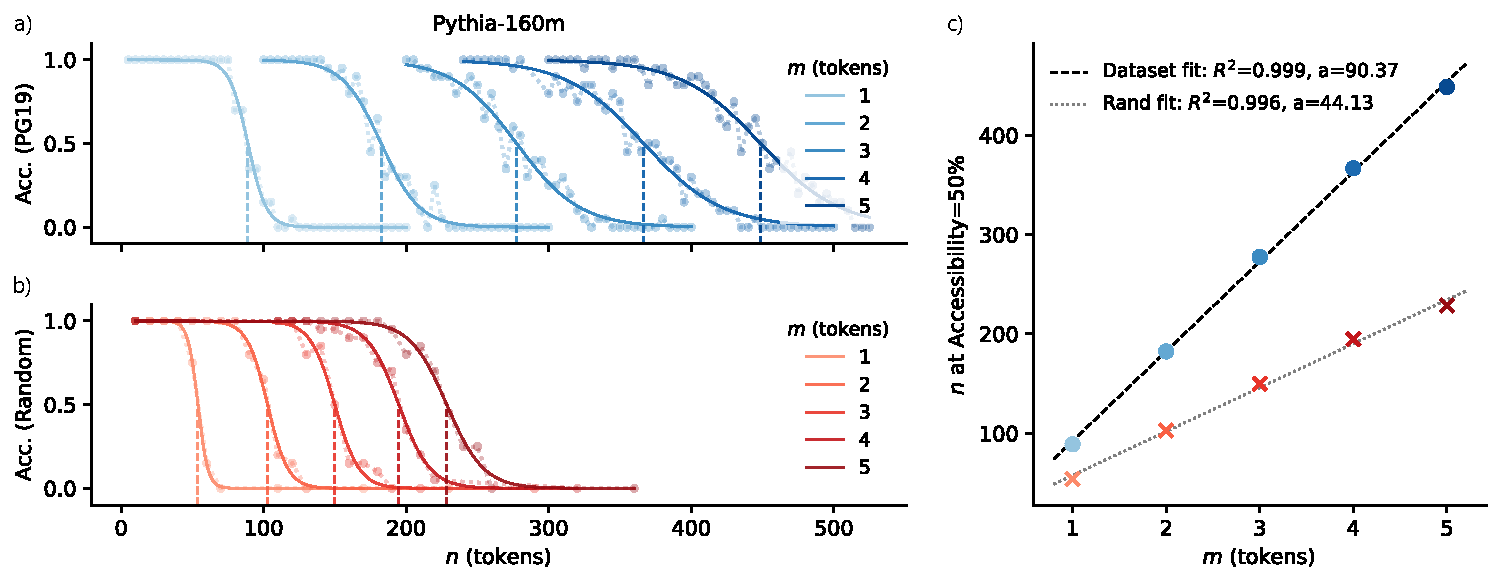
\includegraphics[width=\linewidth]{Images/EleutherAI_pythia-160m_both.pdf}
        \caption{Pythia-160M}
    \end{subfigure}

    \vspace{0.6em}

    \begin{subfigure}[t]{0.95\linewidth}
        \centering
        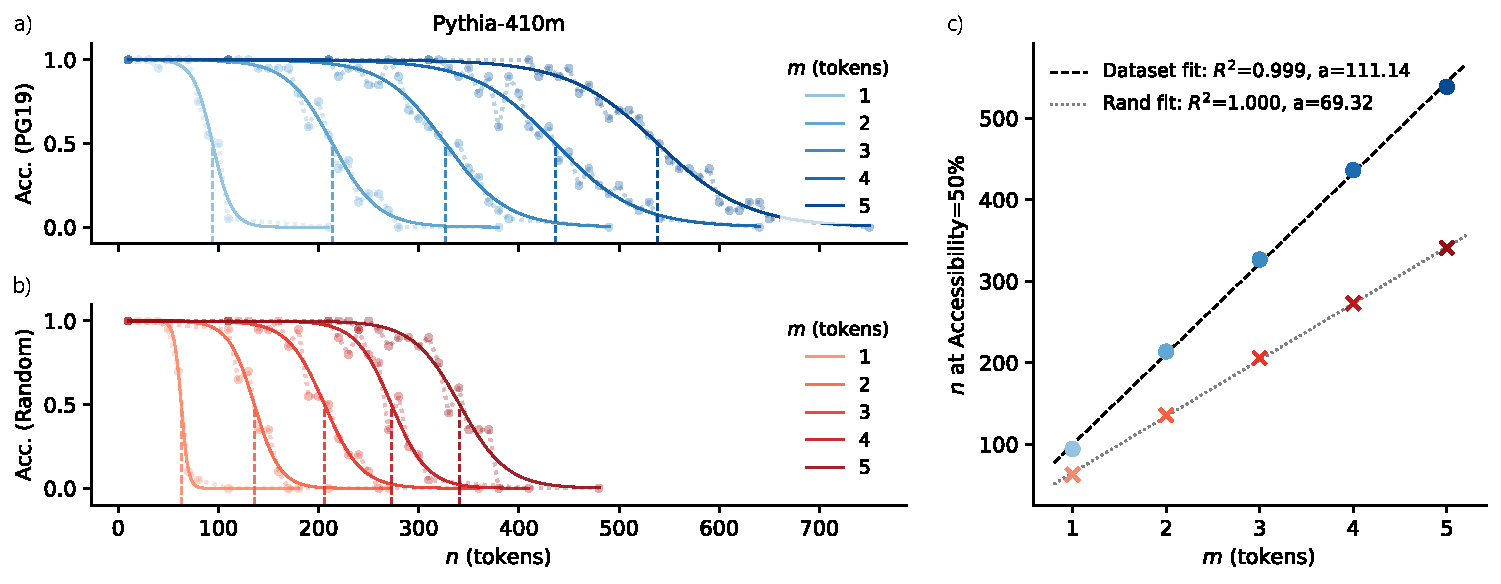
\includegraphics[width=\linewidth]{Images/EleutherAI_pythia-410m_both.pdf}
        \caption{Pythia-410M}
    \end{subfigure}

    \vspace{0.6em}

    \begin{subfigure}[t]{0.95\linewidth}
        \centering
        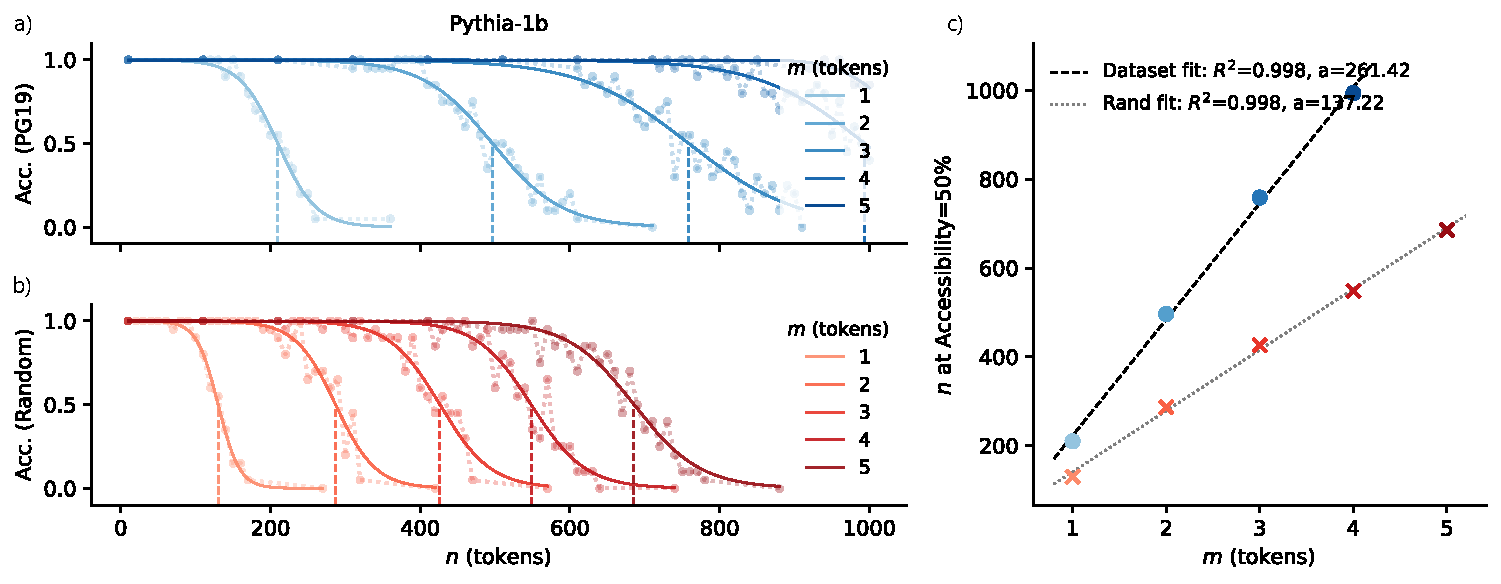
\includegraphics[width=\linewidth]{Images/EleutherAI_pythia-1b_both.pdf}
        \caption{Pythia-1B}
    \end{subfigure}

    \caption{Mean accessibility for a) PG19 and b) random target sequences of length $n$ as a function of the number of trainable memory vectors $m$. For each $m$, we fit a sigmoid (solid) and mark $n_{50}$ where the fit crosses 0.5 (vertical dashed line). (c) $n_{50}(m)$ for PG19 (blue) and random (red), with linear fits (dashed). Results shown for the Pythia model suite at different scales A) 160M, B) 410M, C) 1B.}
    \label{fig:cram_pythia_suite}
\end{figure*}


\begin{figure*}[t]
    \centering

    \begin{subfigure}[t]{0.95\linewidth}
        \centering
        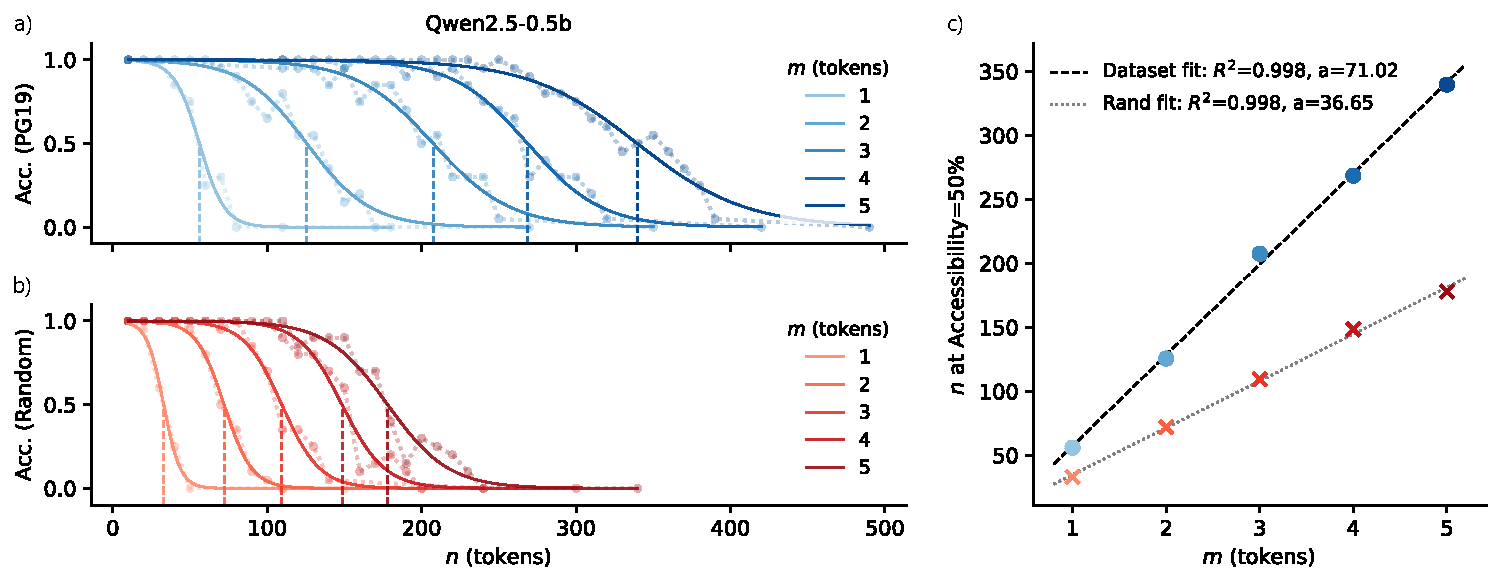
\includegraphics[width=\linewidth]{Images/Qwen_Qwen2.5-0.5B_both.pdf}
        \caption{Qwen 2.5 (0.5B)}
    \end{subfigure}

    \vspace{0.6em}
    
    \begin{subfigure}[t]{0.95\linewidth}
        \centering
        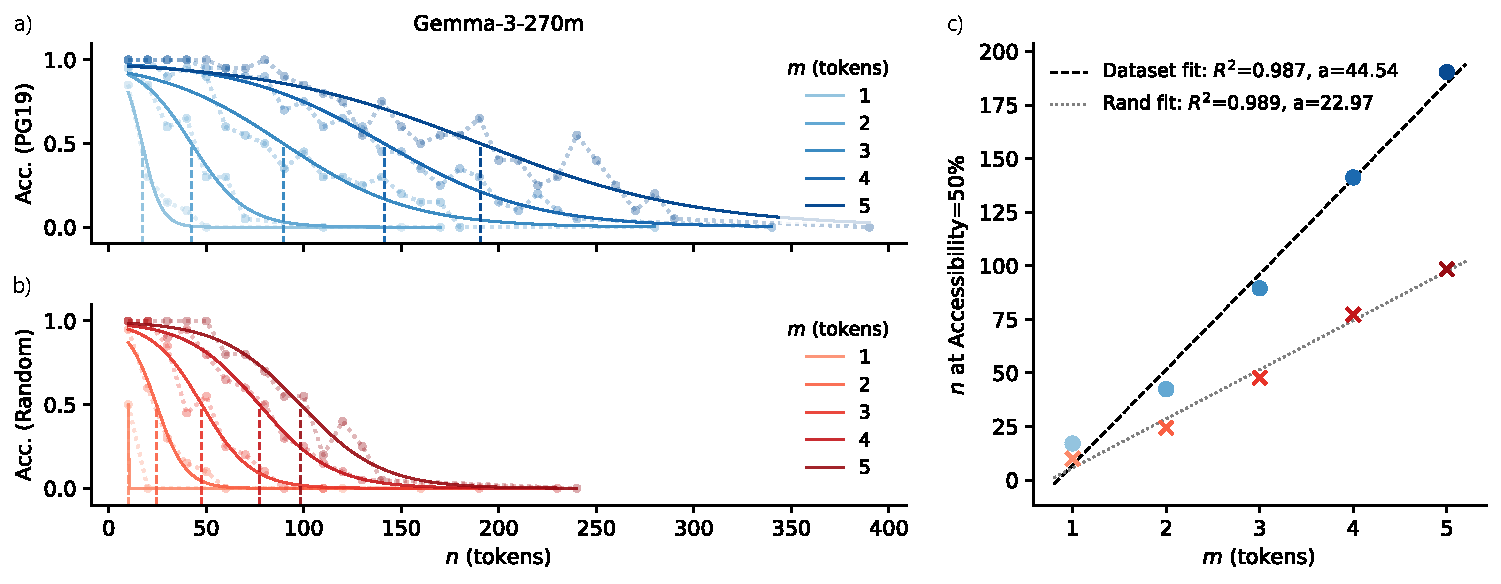
\includegraphics[width=\linewidth]{Images/google_gemma-3-270m_both.pdf}
        \caption{Gemma-3 270M}
    \end{subfigure}

    \vspace{0.6em}


    \begin{subfigure}[t]{0.95\linewidth}
        \centering
        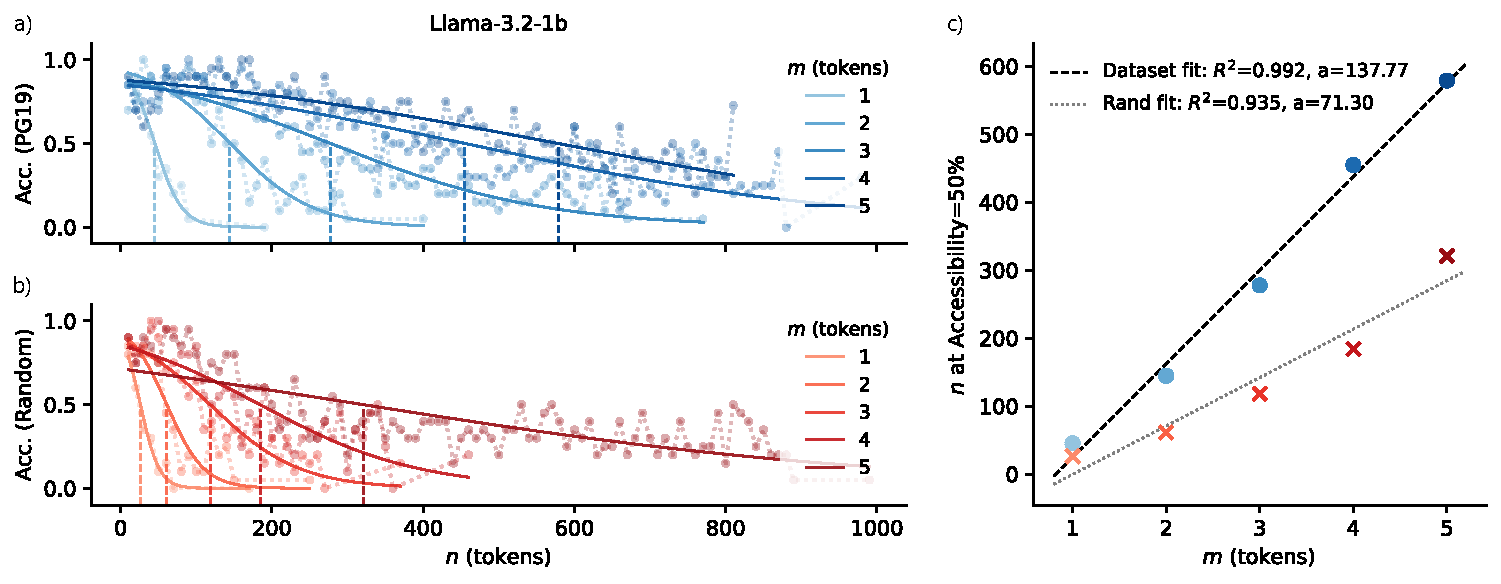
\includegraphics[width=\linewidth]{Images/meta-llama_Llama-3.2-1B_both.pdf}
        \caption{Llama-3.2 1B}
    \end{subfigure}

    \caption{Mean accessibility for a) PG19 and b) random target sequences of length $n$ as a function of the number of trainable memory vectors $m$. For each $m$, we fit a sigmoid (solid) and mark $n_{50}$ where the fit crosses 0.5 (vertical dashed line). (c) $n_{50}(m)$ for PG19 (blue) and random (red), with linear fits (dashed). Results shown for three architectures A) Qwen-2.5, B) Gemma-3, C) Llama-3.2.}
    \label{fig:cram_architectures}
\end{figure*}

\subsection{Support of Different Models}
\label{app:support}

We estimate support parameters for three geometries (Ball, Cone, and Ellipsoid) by Monte Carlo using the sampling procedure described in Section~\ref{sec:support}.
For each sequence length $\ell \in {1,\dots,\ell_{\max}}$, we draw $N=10^5$ i.i.d. token sequences $\textbf{t}^{(k)} = [t_1,\dots,t_\ell]$, where tokens are sampled independently and uniformly as $t_i \sim \mathcal{U}(\{1,\dots,|\mathcal{V}|\})$.
Each sequence is mapped to an embedding vector $Y^{(k)} = (L(\textbf{X}^{(k)}))_{:,-1} \in \mathbb{R}^d$, where $\textbf{X}^{(k)}$ is the embedded input of $\textbf{t}^{(k)}$.

For the Ball baseline, we estimate the $\ell_\infty$ radius \[r = \max_k \|Y_k\|_\infty . \]
For the Cone baseline, we additionally estimate the minimum pairwise cosine similarity to find the opening angle $\theta$
\[c_{\min} = \min_{i<j} \frac{\langle Y_i, Y_j\rangle}{\|Y_i\|_2 \, \|Y_j\|_2},
\qquad \theta = \arccos(c_{\min}) .\]
All support parameters are estimated independently for each $\ell$. We verified empirically that increasing $N$ beyond $10^5$ does not materially change the estimates.

Given $(r,\theta)$, together with the embedding dimension $d$, vocabulary size $|\mathcal{V}|$, and precision $\varepsilon$ defined in Appendix~\ref{app:epsilon}, we compute the theoretical slope proxies used in our plots:
\[
C_{\text{ball}} = \frac{d \log(1 + 2R/\varepsilon)}{\log |\mathcal{V}|},
\qquad
C_{\text{cone}} = \frac{d \log(1 + 2R/\varepsilon) + \log \mathrm{FracCone}(\theta; d)}{\log |\mathcal{V}|}.
\]
with $\mathrm{FracCone}(\theta; d)$ defined as the ratio of packing numbers in Corollary~\ref{cor:cone_pak}.
For the Ellipsoid (axis-aligned rectangle) baseline, we estimate per-coordinate ranges $r_j = \max_{k,k'}|(Y_k)_j - (Y_{k'})_j|$ and use
\[
C_{\text{elli}} = \frac{\sum_{j=1}^d \log(1 + r_j/\varepsilon)}{\log |\mathcal{V}|},
\]

Figure~\ref{fig:support} reports $C_{\text{ball}}$, $C_{\text{cone}}$, and $C_{\text{elli}}$ estimated from samples $\mathbf X_k$ with increasing maximum sequence length $\ell_{\max}$. For all models, the estimated constants stabilize rapidly as $\ell_{\max}$ increases, indicating that short sequences are sufficient to obtain stable estimates of the slope upper bounds.

% Group 2: different architectures (A,B,C) within this figure
\begin{figure*}[t]
    \centering
    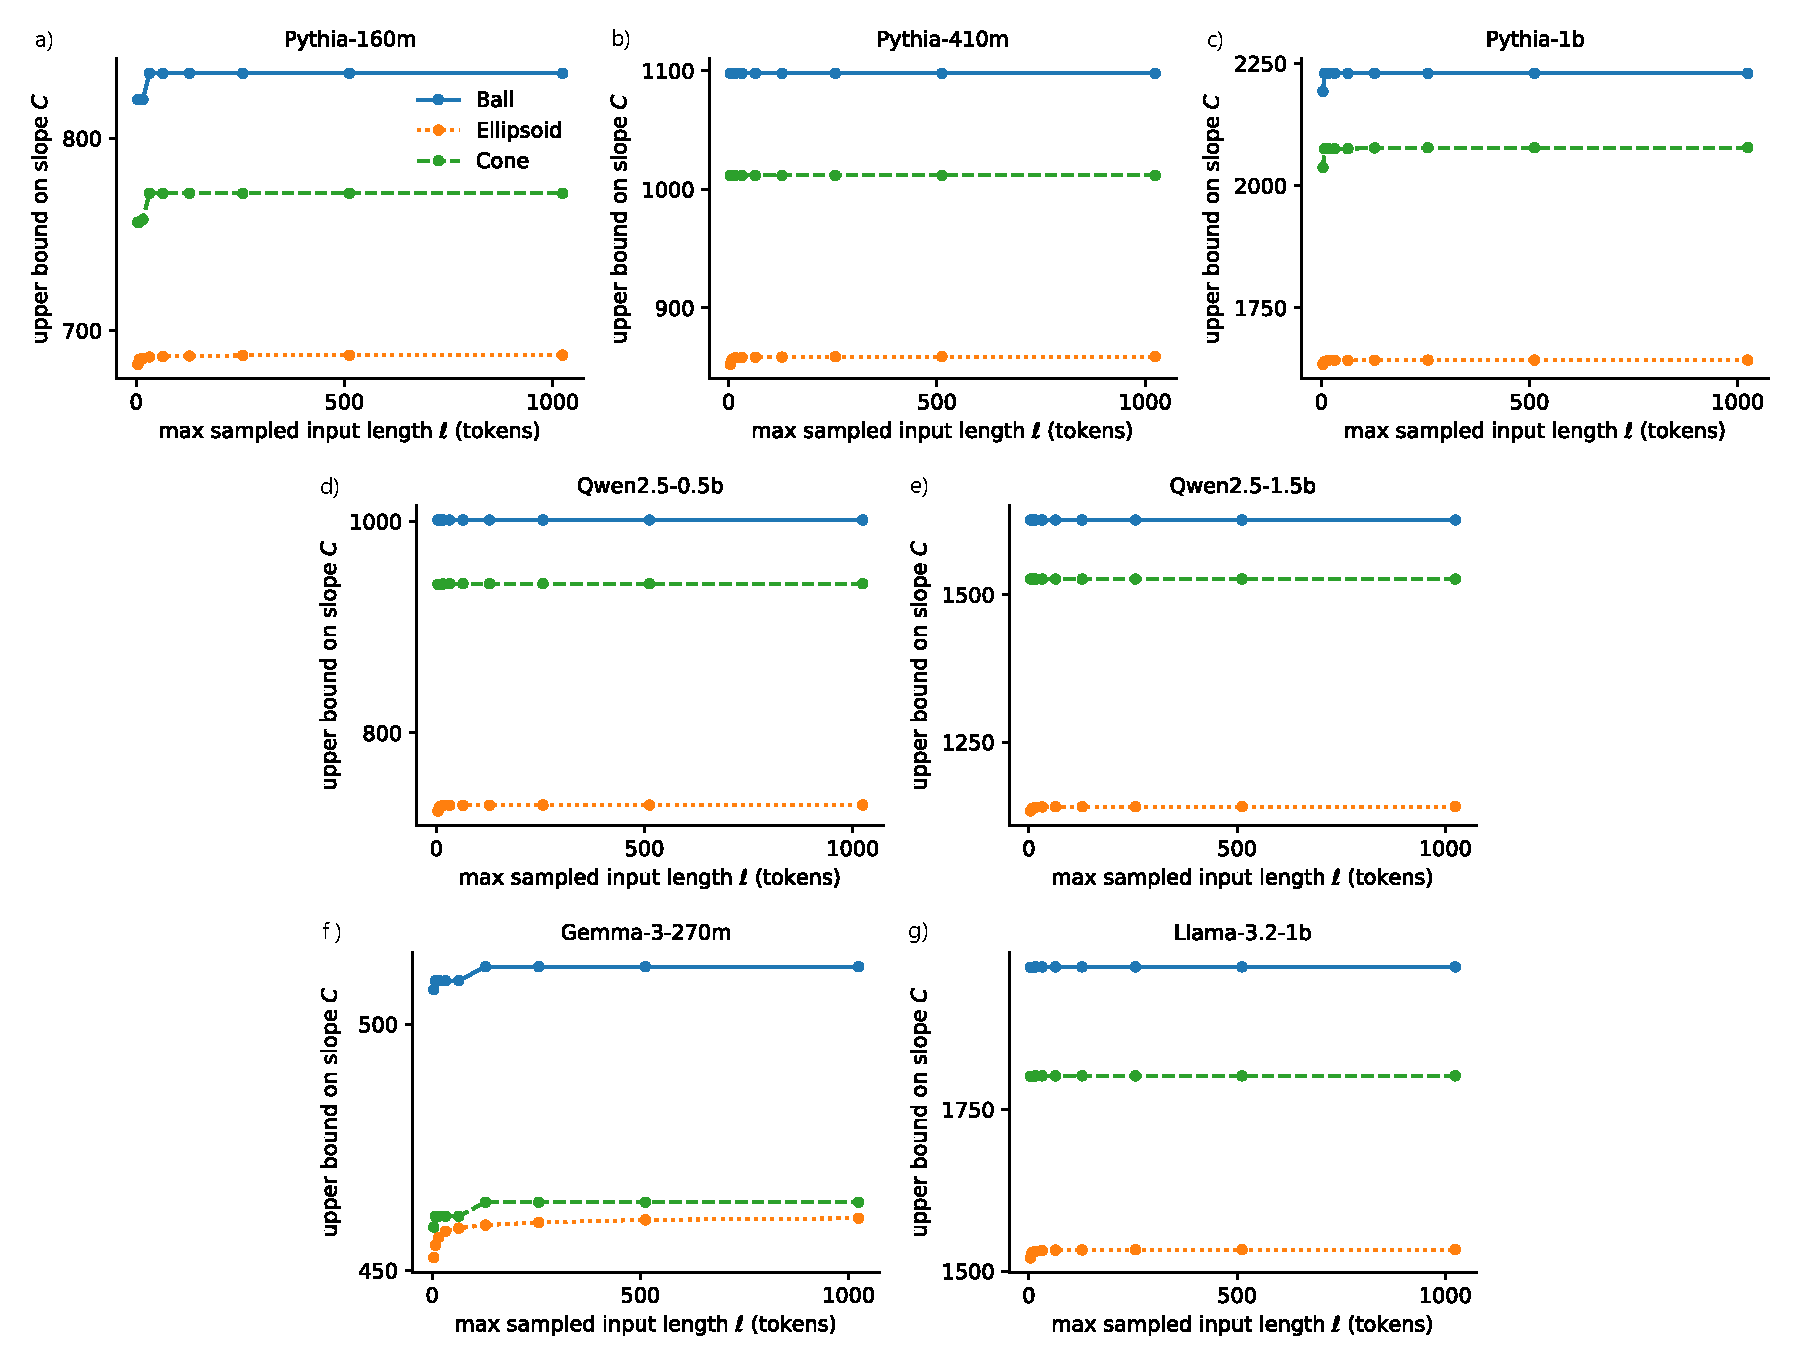
\includegraphics[width=\linewidth]{Images/theoretical_slopes_archi.pdf}
    \caption{Upper bound on $C$ for different support geometry ---Ball (blue), Cone (green), Ellipsoid (orange)---, estimated using 10K randomly sampled input strings of maximum length $\ell$. Sampling prompts longer than $\ell \approx 500$ suffices to estimate the upper bound. Pythia models for different sizes: a) 160M b) 410M, c) 1B and  support for different model architectures d--e) Qwen (0.5B, 1.5B) f) Llama 1B, g) Gemma 270M.}
    \label{fig:support}
\end{figure*}

% \begin{figure*}[t]
%     \centering
%     \includegraphics[width=\textwidth]{Images/supp.pdf}
%     \caption{Cramming experiment for Gemma-3 1b}
%     \label{fig:exp1}
% \end{figure*}

\section{Computing the Cell Volume Distribution}\label{app:cell_vol}

In order to compute the cell volumes $|\mathcal{E}_t|$ corresponding to each token in Section~\ref{sec:cells}, we use the ellipsoid support estimate from Section~\ref{sec:support} and sample points uniformly in volume inside this ellipsoid. (i.e. we sample $\mathbf Y^{(k)} \sim \mathcal{U}([\mathbf x_1^{\min},\mathbf x_1^{\max}]\times \dots \times [\mathbf x_d^{\min}, \mathbf x_d^{\max}])$)
For each sampled point $\mathbf Y^{(k)}$, we compute its greedy token $\hat t^{(k)} = \sigma(\mathbf F\mathbf Y^{(k)})$ via the decoder and count how often each token is selected. 
The relative volume of token $t$ is estimated by
\[
|\mathcal{E}_t|/|\mathcal{E}|
\approx \frac{1}{N}\sum_{k=1}^N \mathbb{I}\{\hat t^{(k)}=t\},
\]
where $\mathcal{E}$ is the support ellipsoid and $N$ is the number of samples (here $N=50$M).

\begin{figure}[t]
    \centering
    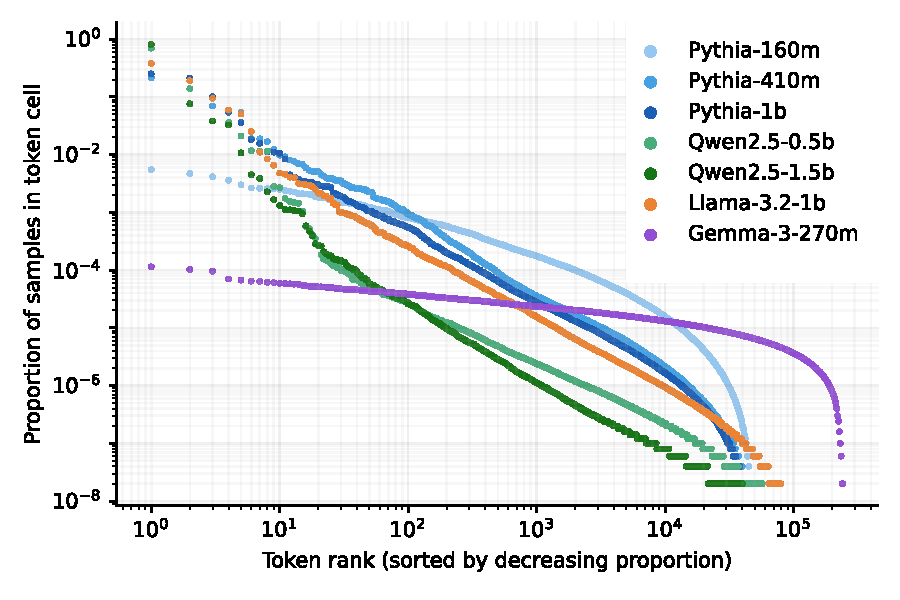
\includegraphics[width=0.50\textwidth]{Images/cell_volume.pdf}
    \caption{Relative volumes of decoder cells across tokens (log-log). For each model, tokens are sorted by estimated cell volume (largest on the left). A small set of tokens (typically $<10^2$) accounts for a large fraction of the support volume, while most tokens ($10^4$--$10^5$) have tiny individual volumes (often $10^{-6}$--$10^{-8}$ of the support).}
    \label{fig:cell_volume}
\end{figure}

Figure~\ref{fig:cell_volume} shows the ranked cell-volume profiles. For most models, volumes are extremely uneven: a small set of tokens takes up a large fraction of the support, while the vast majority of tokens have tiny cells. 
Gemma-3 (and, to a lesser extent, Pythia-160M) looks noticeably more uniform. One possible explanation is their large vocabulary size compared to their number of parameters: if a model has many rare tokens, their decoder embeddings may be weakly trained and remain closer to random. This can lead to a more even partition of the embedding support, with fewer overwhelmingly large cells.
As a sanity check, Table~\ref{tbl:top_tokens} shows that the largest-volume cells in most models align with very frequent tokens (whitespace, punctuation, and common function words). In contrast, Gemma-3 and Pythia-160M have top-volume tokens that appear less obviously frequent, which is consistent with the vocabulary explanation above.

We estimate the distribution of subsequent sequences by using the previously estimated next-token distribution $\mathcal{D}$, and then model the distribution over length-$n$ continuations using the $n$-fold multiplicative convolution $\mathcal{D}^n$. 
Figure~\ref{fig:convolutions_curves} shows the resulting volume-cell distributions for sequence lengths $n \in \{1,\dots,6\}$ across models. 
Most models exhibit highly skewed next-token distributions, leading to a rapid concentration of mass near zero as $n$ increases. 
Models with more balanced distributions, such as Gemma3-270m, exhibit a slower decay.

\begin{table*}[t]
\centering
\small
\caption{Tokens with the largest estimated decoder-cell volumes (Section~\ref{sec:cells}). Volumes are shown in parentheses. Whitespace/control characters are rendered explicitly (e.g., \texttt{\textvisiblespace}, \texttt{\textbackslash n}). For non-ASCII tokens (e.g., Gemma), we show the Unicode code.}
\label{tbl:top_tokens}
\begin{tabular}{l p{0.62\linewidth}}
\toprule
Model & Tokens corresponding to largest cells $\mathcal{E}_t$ ($|\mathcal{E}_t|/|\mathcal{E}|$) \\
\midrule
Pythia-160M &
\texttt{<}$\nu$\texttt{>} ($5.5\mathrm{e}{-3}$), \texttt{<}$\kappa$\texttt{>} ($4.7\mathrm{e}{-3}$), \texttt{<\textvisiblespace>} ($4.1\mathrm{e}{-3}$), \texttt{<|endoftext|>} ($3.9\mathrm{e}{-3}$), \texttt{<well>} ($2.9\mathrm{e}{-3}$)\\
Pythia-410M &
\texttt{<\textbackslash n>} (0.21), \texttt{<,>} (0.08), \texttt{< (>} (0.07), \texttt{<->} (0.06), \texttt{<.>} (0.05)\\
Pythia-1B &
\texttt{<\textbackslash n>} (0.25), \texttt{<,>} (0.21), \texttt{<->} (0.10), \texttt{<.>} (0.054), \texttt{< (>} (0.036)\\
Llama-3.2 1B &
\texttt{<\textvisiblespace>} (0.38), \texttt{<,>} (0.19), \texttt{<\textbackslash n>} (0.094), \texttt{< (>} (0.059), \texttt{<->} (0.051)\\
Qwen-2.5 0.5B &
\texttt{<\textvisiblespace>} (0.70), \texttt{<,>} (0.14), \texttt{<->} (0.038), \texttt{<\textbackslash n>} (0.036), \texttt{<.>} (0.021)\\
Qwen-2.5 1.5B &
\texttt{<\textvisiblespace>} (0.81), \texttt{<,>} (0.076), \texttt{<\textbackslash n>} (0.038), \texttt{<->} (0.033), \texttt{< (>} (0.011)\\
Gemma-3 270M &
\texttt{<eos>} ($1.1\mathrm{e}{-4}$), \texttt{<U+000A U+000A>} ($1.0\mathrm{e}{-4}$), \texttt{</>} ($9.6\mathrm{e}{-5}$), \texttt{<U+3054 U+7406 U+89E3>} ($7.0\mathrm{e}{-5}$), \texttt{<<h2>>} ($6.7\mathrm{e}{-5}$)\\
\bottomrule
\end{tabular}
\end{table*}

\begin{figure}[t]
    \centering
    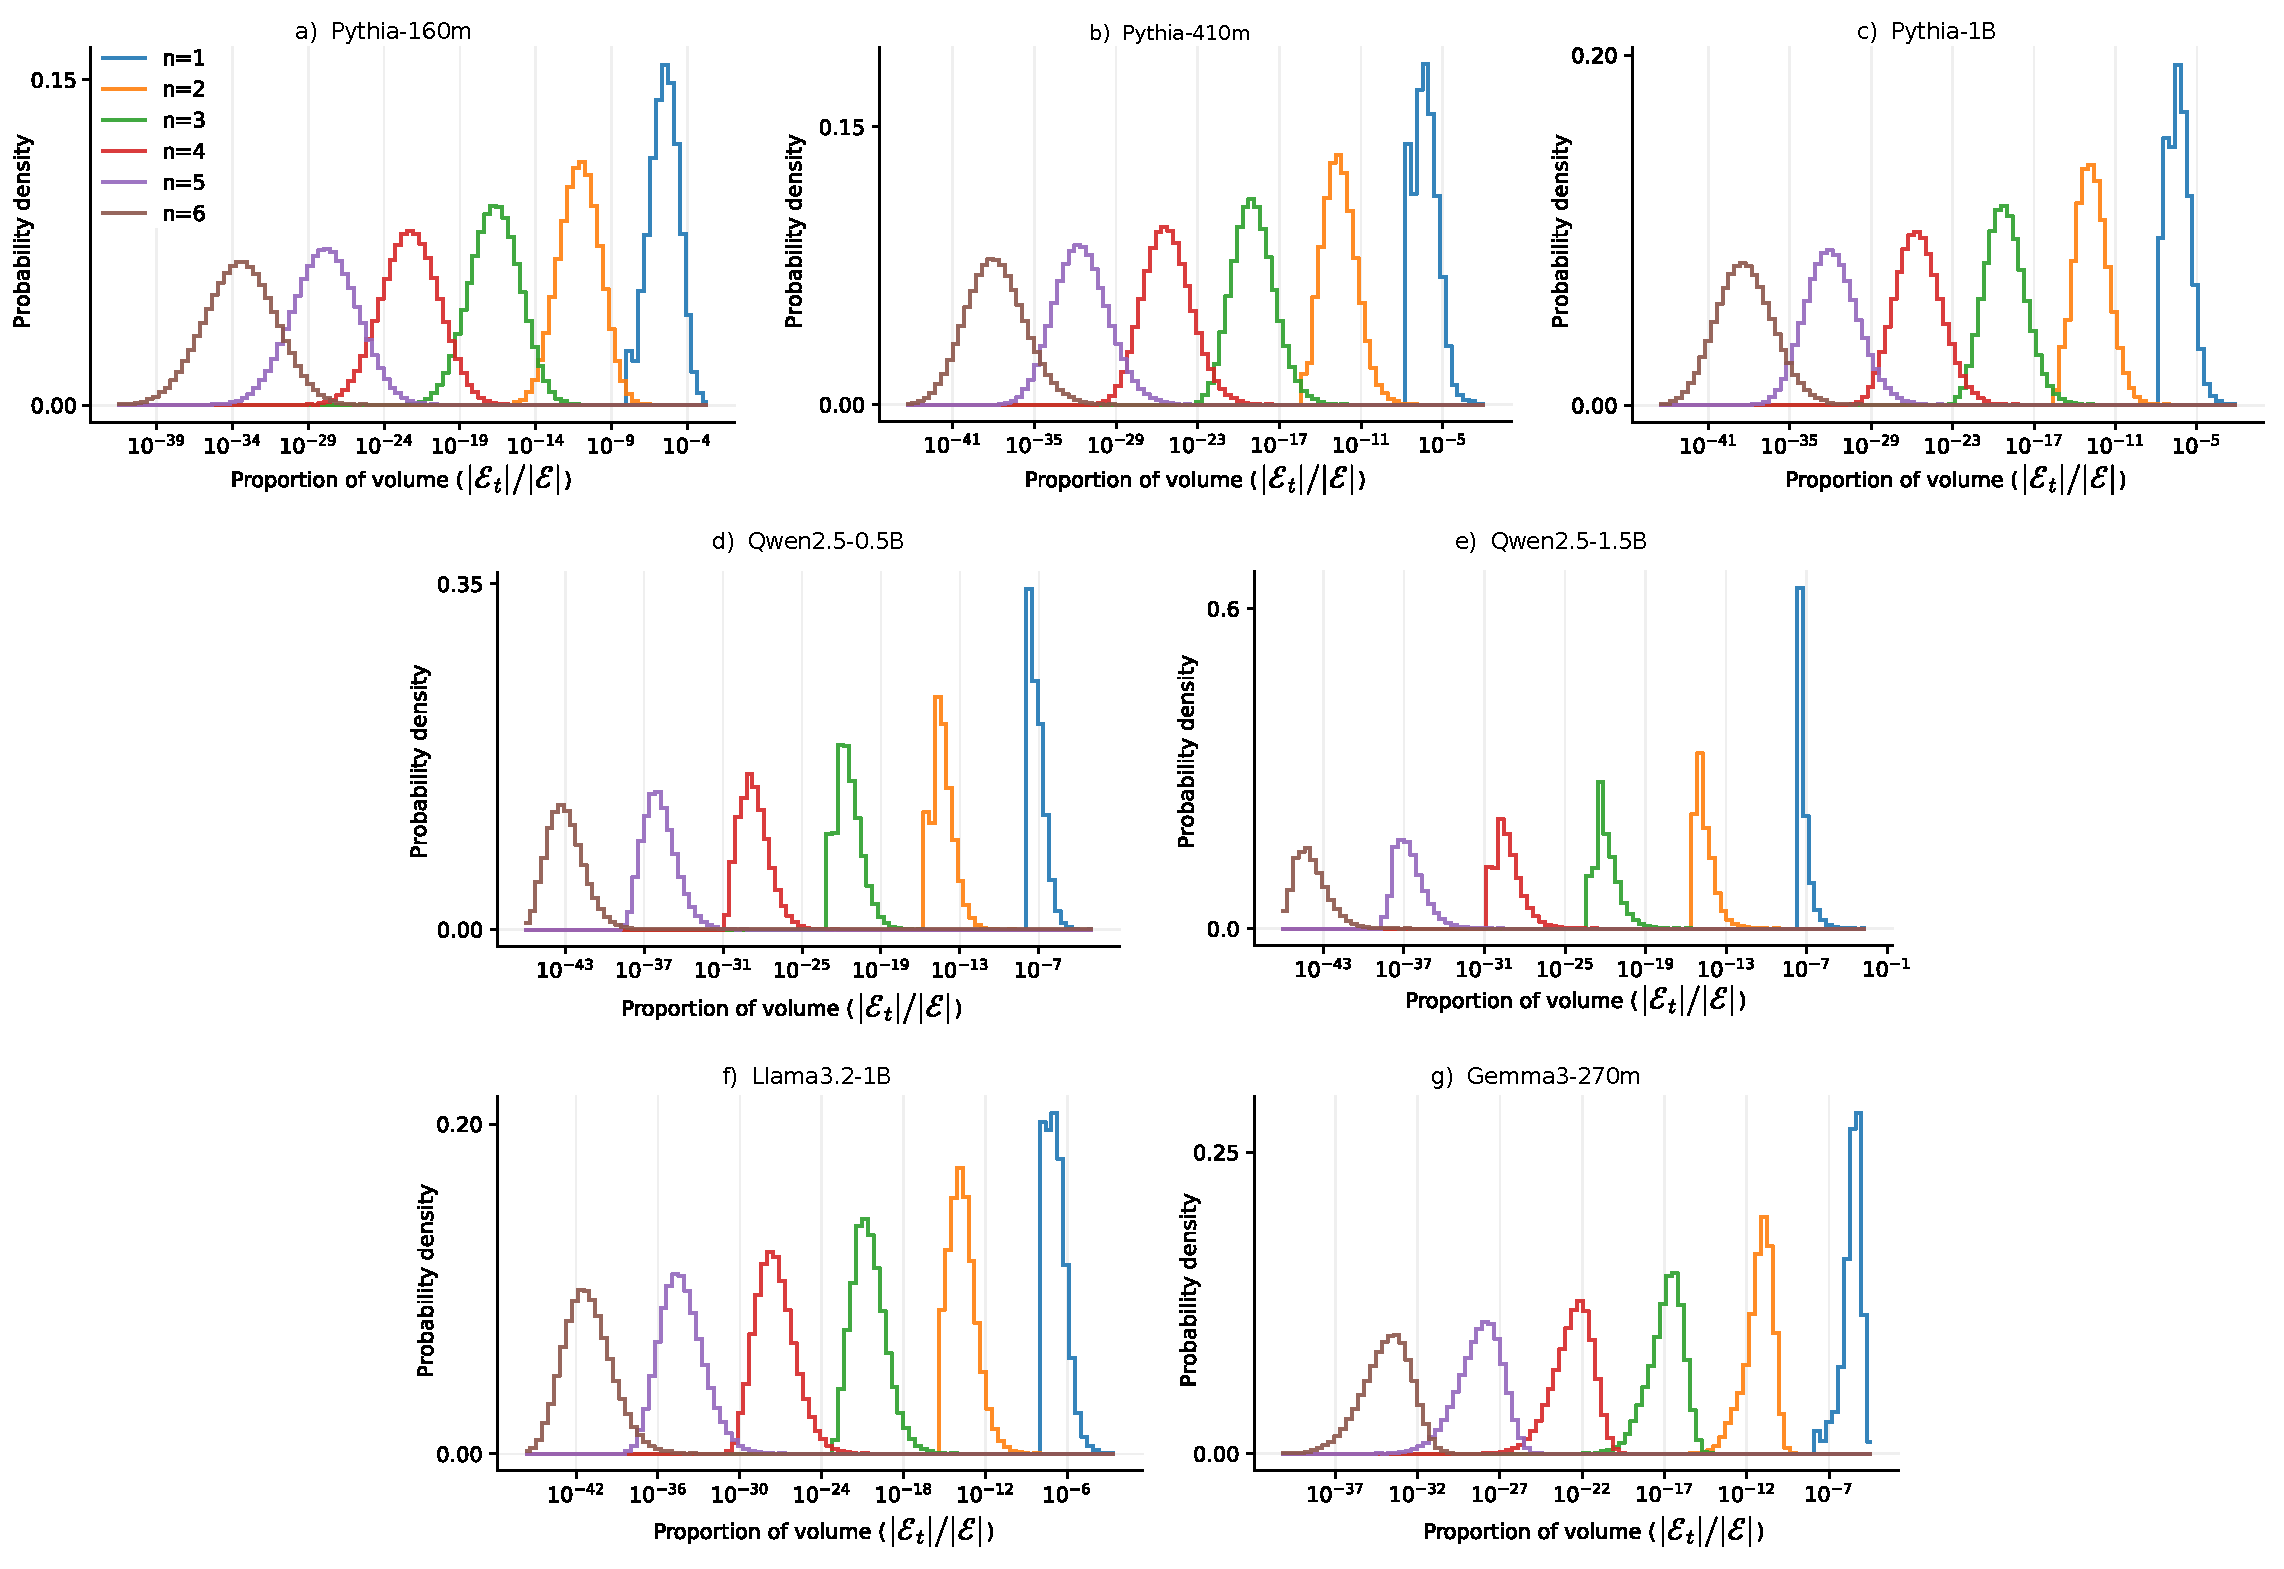
\includegraphics[width=1.0\textwidth]{Images/convolution_curves.pdf}
    \caption{Distribution of $n$-sequences volumes proportions by estimating the $n$-fold convolution of the empirical one-step volume distribution $\mathcal{D}$ for different models: a) Pythia-160M, b) Pythia-410M, c) Pythia-1B, d) Qwen2.5 0.5B, e) Qwen2.5 1.5B, f) Llama3.2 1B, g) Gemma 270M. }
\label{fig:convolutions_curves}
\end{figure}
